\documentclass[8pt]{article}

\usepackage{cheatsheet}
\usepackage{math}

\begin{document}
\begin{multicols*}{4}
    \raggedright
    %! TEX root = ./main.tex

\section{General}

\subsection{Potenzen und Wurzeln}
\begin{itemize}
    \item $a^1 = a$ \textbullet\  $a^0 = 1$
    \item $a^{-n} = \frac{1}{a^n}$
    \item $a^{\frac{1}{n}} = \sqrt[^n]{a}$ \textbullet\ $a^{\frac{m}{n}} = \sqrt[^n]{a^m}$
    \item $a^ma^n = a^{m + n}$
    \item $\frac{a^m}{a^n} = a^{m - n}$
    \item $(a^m)^n = a^{m n}$
    \item $a^nb^n = (ab)^n$
    \item $\frac{a^n}{b^n} = \left( \frac{a}{b} \right)^n$
    \item $a^b = e^{b \ln a}$
    \item $e^{a \ln b} = b^a$
    \item $e^{a + b} = e^a \cdot e^b$
    \item $e^0 = 1$
\end{itemize}

\subsection{Logarithmen}
$y = \log_a x \iff a^x = x$
\begin{itemize}
    \item $a^{\log_a x} = x$
    \item $\log_a a^x = x$
    \item $\log_a a = 1$ \textbullet\ $\log_a 1 = 0$
    \item $\log(uv) = \log(u) + \log(v)$
    \item $\log(\frac{u}{v}) = \log(u) - \log(v)$
    \item $\log(u^r) = r \log(u)$
    \item $\log_a x = \frac{\log_b x}{\log_b a}$
    \item $\ln(a \cdot b) = \ln(a) + \ln(b)$
    \item $\ln(1) = 0$
\end{itemize}

\subsection{Trigonometrische Funktionen}
\begin{itemize}
    \ides{Sinussatz:} $\frac{a}{\sin \alpha} = \frac{b}{\sin \beta} = \frac{c}{\sin \gamma} = 2r$
    \ides{Cosinussatz:} $a^2 = b^2 + c^2 - 2ab \cos \alpha$
    \ides{Tangens:} $\tan(z) := \frac{\sin(z)}{\cos(z)}, z \not\in \{\frac{\pi}{2} + \pi k\}$
    \ides{Cotangens:} $\cot(z) := \frac{\cos(z)}{\sin(z)}, z \not\in \{\pi k\}$
    \item $\exp(iz) = \cos(x) + i \sin(z)$
    \item $\cos(z) = \cos(-z)$ \textbullet\ $\sin(-z) = - \sin(z)$
    \item $\sin(z) = \frac{e^{iz} - e^{-iz}}{2i}$ \textbullet\ $\cos(z) = \frac{e^{iz} + e^{-iz}}{2}$
    \item $\sin(z + w) = \sin(z) \cos(w) + \cos(z) \sin(w)$ \textbullet\ $\cos(z + w) = \cos(z) \cos(w) - \sin(z) \sin(w)$
    \item $\cos(z)^2 + \sin(z)^2 = 1$
    \item $\sin(2z) = 2 \sin(z) \cos(z)$ \textbullet\ $\cos(2z) = \cos(z)^2 - \sin(z)^2 = 1 - 2 \sin^2(z) = 2 \cos^2(z) - 1$
    \item $\tan a = \frac{\sin a}{\cos a}$
    \item $1 + \tan^2 a = \frac{1}{\cos^2 a}$
\end{itemize}

\subsubsection{Komposition}
\resizebox{\columnwidth}{!}{
\begin{tabular}{l l | l l}
    $\sin(\arccos(x)) =$ & $\sqrt{1 - x^2}$ & $\sin(\arctan(x))=$ & $\frac{x}{\sqrt{1 + x^2} }$\\
    $\cos(\arctan(x)) =$ & $\frac{1}{\sqrt{ 1 + x^2}}$ & $\cos(\arcsin(x))=$ & $\sqrt{1 - x^2}$\\
    $\tan(\arcsin(x)) =$ & $\frac{x}{\sqrt{1 - x^2}}$ & $\tan(\arccos(x))$ & $\frac{\sqrt{1 - x^2}}{x}$\\
\end{tabular}}

\subsubsection{Hyperbolisch}
\begin{itemize}
    \item $\sinh = \frac{e^x - e^{-x}}{2}$ \textbullet\ $\cosh = \frac{e^x+e^{-x}}{2}$ \textbullet\ $\tanh = \frac{\sinh(x)}{\cosh(x)}$

    \item $\cosh^2(x) - \sinh^2(x) = 1$
    \item $\sinh(a + b) = \sinh(a)\cosh(b) + \cosh(a)\sinh(b)$
    \item $\cosh(a + b) = \cosh(a)\cosh(b) + \sinh(a)\sinh(b)$
\end{itemize}

\subsubsection{Winkel}
\resizebox{\columnwidth}{!}{
\begin{tabular}{c c c c || c c c c}
    deg   & rad                & $\sin$                 & $\cos$                  & deg & rad & $\sin$ & $\cos$\\\hline
    $0$   & $0$                & $0$                    & $1$                     &
    $30$  & $\frac{\pi}{6}$    & $\frac{1}{2}$          & $\frac{\sqrt{3}}{2}$\\
    $45$  & $\frac{\pi}{4}$    & $\frac{\sqrt{2}}{2}$   & $\frac{\sqrt{2}}{2}$    &
    $60$  & $\frac{\pi}{3}$    & $\frac{\sqrt{3}}{2}$   & $\frac{1}{2}$\\
    $90$  & $\frac{\pi}{2}$    & $1$                    & $0$                     &
    $120$ & $\frac{2\pi}{3}$   & $\frac{\sqrt{3}}{2} $  & $\frac{-1}{2}$\\
    $135$ & $\frac{3 \pi}{4}$  & $\frac{\sqrt{2}}{2}$   & $\frac{-\sqrt{2}}{2}$   &
    $150$ & $\frac{5 \pi}{6}$  & $\frac{1}{2}$          & $\frac{-\sqrt{3}}{2}$\\
    $180$ & $\pi$              & $0$                    & $-1$                    &
    $210$ & $\frac{7\pi}{6}$   & $\frac{-1}{2}$         & $\frac{-\sqrt{3}}{2}$\\
    $225$ & $\frac{5\pi}{4}$   & $\frac{-\sqrt{2}}{2}$  & $\frac{-\sqrt{2}}{2}$   &
    $240$ & $\frac{4\pi}{3}$   & $\frac{-\sqrt{3}}{2}$  & $\frac{-1}{2}$\\
    $270$ & $\frac{3 \pi}{2}$  & $-1$                   & $0$                     &
    $300$ & $\frac{5 \pi}{3}$  & $\frac{-\sqrt{3}}{2} $ & $\frac{1}{2}$\\
    $315$ & $\frac{7 \pi}{4}$  & $\frac{-\sqrt{2}}{2} $ & $\frac{\sqrt{2}}{2}$    &
    $330$ & $\frac{11 \pi}{6}$ & $\frac{-1}{2} $        & $\frac{\sqrt{3}}{2}$\\
\end{tabular}}

\resizebox{\columnwidth}{!}{
\begin{tabular}{l | l | l}
    $\arcsin(0) = 0$                & $\arccos(0) = \frac{\pi}{2}$ & $\arctan(0) = 0$\\
    $\arcsin(1) = \frac{\pi}{2}$    & $\arccos(0) = 0$             & $\arctan(1) = \frac{\pi}{4}$\\
    $\arcsin(-1) = -\frac{\pi}{2}$  & $\arccos(0) = \pi$           & $\arctan(-1) = -\frac{\pi}{4}$\\
                                    &                               & $\arctan(\sqrt{3}) = \frac{\pi}{3}$\\
\end{tabular}}

\begin{itemize}
    \item $\arccos(x) = \frac{\pi}{2} - \arcsin(x)$
\end{itemize}

\subsubsection{Reduktion}
\resizebox{\columnwidth}{!}{\begin{tabular}{l | l | l}
    $\sin \frac{\pi}{2} - a = \cos a$ & $\cos \frac{\pi}{2} - a = \sin a$ & $\tan \frac{\pi}{2} - a = \frac{1}{\tan a}$\\
    $\sin \frac{\pi}{2} + a = \cos a$ & $\cos \frac{\pi}{2} + a = -\sin a$ & $\tan \frac{\pi}{2} + a = \frac{-1}{\tan a}$\\
    $\sin \pi - a = \sin a$ & $\cos \pi - a = -\cos a$ & $\tan \pi - a = -\tan a$\\
    $\sin \pi + a = -\sin a$ & $\cos \pi + a = -\cos a$ & $\tan \pi + a = \tan a$\\
    $\sin 2\pi -a = -\sin a$ & $\cos 2\pi - a = \cos a$ & $\tan 2 \pi - a = -\tan a$\\
    $\sin -a = -\sin a$ & $\cos - a = \cos a$ & $\tan - a = -\tan a$\\
\end{tabular}}

\subsection{Sonstiges}
\begin{itemize}
    \ides{Mitternacht:} $x_{1 / 2} = \frac{-b \pm \sqrt{b^2 - 4ac}}{2a}$
    \item $\sqrt{i} = \frac{\sqrt{2}}{2} + i \frac{\sqrt{2}}{2}$
    \ides{Ellipse Gleichung:} $\frac{x^2}{a^2} + \frac{y^2}{b^2} = 1$
    \ides{Ellipse Volumen:} $\pi a b$
\end{itemize}

\subsection{Komplexe Zahlen}
\begin{itemize}
    \ides{Imaginary Number:} $i, i^2 = -1$
    \ides{Complex Number:} $z, z = x + iy, \ x, y \in \R$
    \ides{Set:} $\C = \{x + iy | x,y \in \R\}$
    \ides{Konjugate:} $\overline{z} = x - iy, \ z = x + iy$
        \begin{itemize}
            \item $z \cdot \overline{z} = x^2 \cdot y^2 = |z|^2$
            \item $\overline{z_1 + z_2} = \overline{z_1} + \overline{z_2}$
            \item $\overline{z_1 \cdot z_2} = \overline{z_1} \cdot \overline{z_2}$
        \end{itemize}
    \ides{Betrag:} $|z|$ Distanz zwischen $z$ und Origin
        \begin{itemize}
            \item $|z| = \sqrt{x^2 + y^2} = \sqrt{z \cdot \overline{z}} $
            \item $|z| = |\overline{z}|$
            \item $|z_1 + z_2| \le |z_1| + |z_2|$
            \item $|z_1 \cdot z_2| = |z_1||z_2|$
            \item $|\frac{z_1}{z_2}| = \frac{|z_1|}{|z_2|}$
        \end{itemize}
    \ides{Euler:} $e^{i\gamma} = \cos \gamma + i \sin \gamma$
        \begin{itemize}
            \item $|e^{i \gamma}| = 1$
        \end{itemize}
\end{itemize}

\subsubsection{Arithmetic}
Für $z_1 = a + ib = re^{i \gamma}, z_2 = b + id = se^{i \delta}$:
\begin{itemize}
    \item $z_1 + z_2 = (a + ib) + (c + id) = (a + c) + i(b + d)$
    \item $z_1 \cdot z_2 = (a + ib) \cdot (c + id) = (ac - bd) + i(ad + bc)$
        \begin{itemize}
            \item $z_1 z_2 = rse^{i(\gamma + \delta)}$
        \end{itemize}
    \item $\frac{z_1}{z_2} = \frac{z_1 \cdot \overline{z_2}}{z_2 \cdot \overline{z_2}}= \frac{z_1 \cdot \overline{z_2}}{|z_2|}$
        \begin{itemize}
            \item $\frac{z_1}{z_2} = \frac{r}{s}e^{i(\gamma - \delta)}$
        \end{itemize}
        \item $\sqrt[^n]{z_1} = z_2 \implies z_1 = z_2^n = r^ne^{i n \delta} \overset{!}{=} re^{i\gamma}$
            \begin{itemize}
                \item $s = \sqrt[^n]{r}$
                \item $n \gamma = \gamma + 2 \pi k, k = 0\dots n - 1$
            \end{itemize}
\end{itemize}

\subsubsection{Polar Coordinates}
$z = x + iy \iff z = r(\cos \gamma + i \sin \gamma) \overset{Euler}{=} z = r e^{i \gamma}$
\begin{itemize}
    \item $x = r \cos \gamma$ \textbullet\ $y = r \sin \gamma$
    \item $r = |z|$
    \item $\gamma = \arccos \frac{x}{r} = \arcsin \frac{y}{r}$
    \item $\text{arg}z = |z| \in [0, 2\pi[ \implies r$ ist eindeutig bestimmt
\end{itemize}

\subsection{Rechenregeln Ableitung}
\begin{itemize}
    \ides{$\mathbf{f + g}$:} $(f + g)'(x_0) = f'(x_0) + g'(x_0)$.
    \ides{$\mathbf{f \cdot g}$:} $(f \cdot g)'(x_0) = f'(x_0)g(x_0) + f(x_0)g'(x_0)$.
    \ides{$\mathbf{\frac{f}{g}}$:} $\left( \frac{f}{g} \right)' (x_0) = \frac{f'(x_0)g(x_0) - f(x_0)g'(x_0)}{g(x_0)^2}, \ g(x_0) \neq 0$.
    \ides{$\mathbf{g \circ f}$:} $(g \circ f)'(x_0) = g'(f(x_0)) \cdot f'(x_0)$
\end{itemize}

\subsection{Rechenregel Integral}
\begin{itemize}
    \ides{Partiell:} $\int_{a}^{b} f(x)g'(x) \mathrm{d}x = f(x)g(x)|_a^b - \int_{a}^{b} f'(x)g(x) \mathrm{d}x$
    \ides{Substitution:} $\int_{\phi(a)}^{\phi(b)} f(x) \mathrm{d}x = \int_a^b f(\phi(t))\phi'(t) \mathrm{d}t$
\end{itemize}

\subsection{Bekannte Reihen}
\resizebox{\columnwidth}{!}{\begin{tabular}{l | l | c | c | c}
    \multicolumn{2}{l |}{Reihe}                                      & Wert                                   & konv.               & div.\\\hline
    \multicolumn{2}{l |}{Geometrische Reihe}                         & $q \in \C$                             &                     & \\\hline
    $\sum_{k=0}^{\infty} aq^k$                                       & $a + aq +$                             & $\frac{a}{1-q}$     & $|g| < 1$    & $|q| \ge 1$\\\hline
    $\sum_{k=0}^{\infty} (k+1)q^k$                                   & $1 + 2q +$                             & $\frac{1}{(1-q)^2}$ &              & \\\hline
    \multicolumn{2}{l |}{Harmonische Reihe}                          &                                        &                     & \\\hline
    $\sum_{k=1}^{\infty} \frac{1}{k}$                                &                                        & $\infty$            &              & \\\hline
    $\sum_{k=1}^{\infty} \frac{1}{k^2}$                              &                                        & $\frac{\pi^2}{6}$   &              & \\\hline
    $\sum_{k=1}^{\infty} \frac{1}{k^4}$                              &                                        & $\frac{\pi^4}{90}$  &              & \\\hline
    $\sum_{k=1}^{\infty} \frac{1}{k^a}$                              &                                        &                     & $a > 1$      & $a \le 1$\\\hline
    \multicolumn{2}{l |}{Alternierende Harmon. Reihe}                &                                        &                     & \\\hline
    $\sum_{k=1}^{\infty} \frac{(-1)^{k+1}}{k}$                       &                                        & $\ln 2$             &              & \\\hline
    $\sum_{k=1}^{\infty} \frac{(-1)^{k+1}}{k^2}$                     &                                        & $\frac{\pi^2}{12}$  &              & \\\hline
    $\sum_{k=1}^{\infty} \frac{(-1)^{k+1}}{k^4}$                     &                                        & $\frac{\pi^4}{720}$ &              & \\\hline
    $\sum_{k=0}^{\infty} \frac{(-1)^k}{2k + 1}$                      & $1 - \frac{1}{3} + \frac{1}{5} -$      & $\frac{\pi}{4}$     &              & \\\hline
    \multicolumn{1}{l |}{Teleskopreihe}                              &                                        &                     & \\\hline
    $\sum_{k=1}^{\infty} \frac{1}{k(k+1)}$                           &                                        & $1$                 &              & \\\hline
    \multicolumn{3}{l |}{Exponentialfunktion $z \in \C,$ konv. abs.} &                                        & \\\hline
    $\sum_{k=0}^{\infty} \frac{z^k}{k!}$                             & $1 + z + \frac{z^2}{2!} +$             & $\exp{z}$           &              & \\\hline
    $\sum_{k=0}^{\infty} \frac{(-a)^k}{k!}$                          &                                        & $\frac{1}{e^a}$       &              & \\\hline
    $\sum_{k=0}^{\infty} (-1)^k\frac{x^{2k+1}}{(2k+1)!}$             & $x -\frac{x^3}{3!} + \frac{x^5}{5!} -$ & $ \sin x$           &              & \\\hline
    $\sum_{k=0}^{\infty} (-1)^k\frac{x^{2k}}{(2k)!}$                 & $1-\frac{x^2}{2}+\frac{x^4}{4!}-$      & $\cos x$            &              & \\\hline
    $\sum_{k=0}^{\infty} \frac{x^{2k+1}}{(2k+1)!}$                   & $x+\frac{x^3}{3!}+\frac{x^5}{5!}+$     & $\sinh x$           &              & \\\hline
    $\sum_{k=0}^{\infty} \frac{x^{2k}}{(2k)!}$                       & $1+\frac{x^2}{2}+\frac{x^4}{4!}+$      & $\cosh x$           &              & \\\hline
\end{tabular}}

\subsection{Spezielle Summen}
\resizebox{\columnwidth}{!}{
\begin{tabular}{l | l | c}
    $\sum_{k=1}^{n} k$ & $1 + 2 + \dots + n$ & $\frac{n(n+1)}{2}$\\\hline
    $\sum_{k=1}^{n} k^2$ & $1 + 4 + \dots + n^2$ & $\frac{n(n+1)(2n+1)}{6}$\\\hline
    $\sum_{k=1}^{n} k^3$ & $1 + 8 + \dots n^3$ & $\left( \sum_{k=1}^{\infty} k  \right)^2$\\\hline
    $\sum_{k=1}^{n} (2k - 1)$ & $1 + 3 + \dots + (2n -1)$ & $n^2$\\\hline
    $\sum_{k=1}^{n} (2k - 1)^2$ & $1 + \dots + (2n - 1)^2$ & $\frac{n(2n-1)(2n+1)}{3}$\\\hline
    $\sum_{k=0}^{n-1} q^k$ & $1 + q + \dots = \frac{q^n-1}{q-1}$ & $\frac{1 - q^n}{1-q}, \ q \not\in \{0, 1\}$\\\hline
\end{tabular}}

\subsection{Funktionen und deren Grenzwert}
\resizebox{\columnwidth}{!}{
\begin{tabular}{l | c | c}
    Funktion & Grenzwert & Bedingung\\\hline
    $\lim_{n \to \infty} a^n$ & $0$ & $|a| < 1$\\\hline
    $\lim_{n \to \infty} \sqrt[^n]{a}$ & $1$ & $a > 0$\\\hline
    $\lim_{n \to \infty} \sqrt[^n]{n^a}$ & $1$ & $a > 0$\\\hline
    $\lim_{n \to \infty} \sqrt[^n]{n}$ & $1$\\\hline
    $\lim_{n \to \infty} \frac{\log_an}{n}$ & $0$ & $a > 1$\\\hline
    $\lim_{n \to \infty} \frac{n^k}{a^n}$ & $0$ & $a > 1$\\\hline
    $\lim_{n \to \infty} \frac{a^n}{n!}$ & $0$\\\hline
    $\lim_{n \to \infty} \sum_{k=1}^{n} \frac{1}{k}$ & $\infty$\\\hline
    $\lim_{n \to \infty} \left( 1 + \frac{1}{n} \right)^n$ & $e$\\\hline
    $\lim_{n \to \infty} \left( 1 + \frac{a}{n} \right)^n$ &e$^a$\\\hline
    $\lim_{n \to \infty} \left( 1 - \frac{1}{n} \right)^n$ & $\frac{1}{e}$\\\hline
    $\lim_{n \to 0} \frac{\sin n}{n}$ & $1$\\\hline
    $\lim_{n \to 1} \frac{\ln n}{n - 1}$ & $1$\\\hline
    $\lim_{n \to \infty} \frac{n^m}{\exp(an)}$ & $0$ & $m \in \R, a > 0$\\\hline
    $\lim_{n \to 0} \frac{\exp(n) - 1}{n}$ & $1$\\\hline
    $\lim_{n \to 0} \frac{\ln(1 + n)}{n}$ & $1$\\\hline
    $\lim_{n \to \infty} \frac{\ln n}{n^a}$ & $0$ & $a > 0$\\\hline
    $\lim_{n \to 0} \frac{a^n - 1}{n}$ & $\ln a$ & $a > 0$\\\hline
    $\lim_{n \to 0} (n^a \ln n)$ & $0$ & $a > 0$\\\hline
\end{tabular}}

\subsection{Auf- und Ableitungen}
\resizebox{\columnwidth}{!}{
\begin{tabular}{l | l | l}
    $f'(x)$ & $f(x)$ & $F(x)$\\
    \hline
    $sax^{s-1}$                                                       & $ax^s$                  & $\frac{a}{s + 1}x^{s + 1}$\\
    $\frac{1}{x}$                                                     & $\ln(ax)$               & $x \ln(ax) - x$\\
    $\frac{1}{x + a}$                                                 & $\ln(x + a)$            & $(x + a) \ln(x + a) + x$\\
    $ae^{ax}$                                                         & $e^{ax}$                & $\frac{1}{a} e^{ax}$\\
    $\frac{-a}{x^2}$                                                  & $\frac{a}{x}$           & $a\ln(|x|)$\\
    $\ln(a)b a^{b x}$                                                 & $a^{bx}$                & $\frac{a^{bx}}{\ln(a)b}$\\
    $\frac{1}{2\sqrt{x}}$                                             & $\sqrt{x}$              & $\frac{2}{3}x^{3/2}$\\
    $\frac{1}{x\ln(a)}$                                               & $\log_a(x)$             & $\frac{x(\ln(x)-1)}{\ln(a)}$\\
    $\cos(x)$                                                         & $\sin(x)$               & $-\cos(x)$\\
    $\frac{1}{\sqrt{1-x^2} }$                                         & $\arcsin(x)$            & $x \arcsin(x) + \sqrt{1 - x^2}$\\
    $2 \sin(x) \cos(x)$                                               & $\sin^2(x)$             & $\frac{x - \sin(x) \cos(x)}{2}$\\
    $-\sin(x)$                                                        & $\cos(x)$               & $\sin(x)$\\
    $\frac{-1}{\sqrt{1-x^2} }$                                        & $\arccos(x)$            & $x \arccos(x) - \sqrt{1 - x^2}$\\
    $-2 \sin(x) \cos(x)$                                              & $\cos^2(x)$             & $\frac{x + \sin(x) \cos(x)}{2}$\\
    $\frac{1}{\cos^2(x)} =$                                           & $\tan(x)$               & $-\ln(|\cos(x)|)$\\
    $1 + \tan^2(x)$                                                   &                         & \\
    $\frac{1}{1+x^2}$                                                 & $\arctan(x)$            & $x \arctan(x) - \frac{\ln(x^2 + 1)}{2}$\\
    $2a(\cos(ax))^2-a$                                                & $\sin(ax) \cos(ax)$     & $-\frac{1}{4a}\cos(2ax) =$\\
                                                                      &                         & $\frac{-(\cos^2(ax))}{2a}$\\
                                                                      & $\sin(x) \sin^2(x)$     & $\frac{-\sin^2(x) - 2}{3}\cos(x)$\\
                                                                      & $\cos(x) \cos^2(x)$     & $\frac{\sin(x) \cos^2(x) + 2 \sin(x)}{3}$\\
                                                                      & $\sin(x) \cos^2(x)$     & $\frac{-\cos^3(x)}{3}$\\
                                                                      & $\sin^2(x) \cos(x)$     & $\frac{\sin^3(x)}{3}$\\
                                                                      & $\sin(x) \sin(2x)$      & $\frac{-\sin(3x) + 3 \sin(x)}{6}$\\
                                                                      & $\cos(x) \cos(2x)$      & $\frac{\sin(3x) + 3 \sin(x)}{6}$\\
    $\frac{2x}{(x^2 + 1)^2}$                                          & $\frac{x^2}{x^2 + 1}$   & $x - \arctan(x)$\\
    $\frac{-4x}{(x^2 + 1)^3}$                                         & $\frac{1}{(1 + x^2)^2}$ & $\frac{x}{2x^2 + 2} + \frac{\arctan(x)}{2}$\\
                                                                      & $\frac{u'(x)}{u(x)}$    & $\ln |u(x)|$\\
                                                                      & $u'(x) \cdot u(x)$      & $\frac{1}{2}(u(x)^2)$\\
\end{tabular}}

\resizebox{\columnwidth}{!}{
\begin{tabular}{l | l | l}
    $\frac{-x}{\sqrt{a^2 - x^2}}$                                     & $\sqrt{a^2 - x^2}$      & $\frac{a^2 \arcsin(\frac{x}{|a|})+ x \sqrt{a^2 - x^2}}{2}$\\
    $\frac{x}{\sqrt{x^2 + a^2}}$                                      & $\sqrt{a^2 + x^2}$      & $\frac{a^2 \ln(| \sqrt{x^2 + a^2} +x|) + x \sqrt{a^2 + x^2}}{2}$\\
    $x^x (1 + \ln x)$                                                 & $x^x$                   & \\
    $e^{\ln |x|}(\ln(|x|) + 1)$                                       & $|x|^x = e^{x \ln x}$   & \\
    $\frac{-2}{(x + a)^3}$                                            & $\frac{1}{(x + a)^2}$   & $\frac{-1}{x + a}$\\
    $\cosh(x)$                                                        & $\sinh(x)$              & $\cosh(x)$\\
    $\frac{1}{\sqrt{1+x^2}}$                                          & $\arcsinh(x)$           & \\
    $\sinh(x)$                                                        & $\cosh(x)$              & $\sinh(x)$\\
    $\frac{1}{\sqrt{x-1}\sqrt{x+1}}$                                  & $\arccosh(x)$           & \\
    $\frac{1}{\cosh^2(x)} =$                                          & $\tanh(x)$              & $\ln(e^{2x} + 1) - x$\\
    $1 - \tanh^2(x)$                                                  &                         & \\
    $\frac{1}{2x+2} - \frac{1}{2x - 2}$                               & $\arctanh(x)$           & \\
\end{tabular}}

\subsection{Kombinatorik}
\begin{itemize}
    \item Anzahl Permutation ohne Wiederholung: $n!$
    \item Anzahl der Kombinationen ohne Wiederholung: ${n\choose k} = \frac{n!}{k!(n - k)!}$
    \item Anzahl Variationen mit Wiederholung: $n^m$
\end{itemize}

    \clearpage
    \part{Wahrscheinlichkeiten}
    %! TEX root = ./main.tex

\section{Wahrscheinlichkeit}
\subsection{Grundbegriffe}
\begin{itemize}
    \ides{Ereignisraum $\bs{\Omega}$:} Menge aller möglichen Ergebnisse des Zufallsexperiments
        \begin{itemize}
            \item $\Omega \neq \emptyset$
        \end{itemize}
    \ides{Elementarereignisse $w \in \Omega$:} Element aus Ereignisraum
    \ides{Potenzmenge $2^\Omega$:} von $\Omega$ ist die Menge aller Teilmengen von $\Omega$
    \ides{Ereignis $A \in 2^\Omega$:} Element der Potenzmenge
        \begin{itemize}
            \item $A$ tritt ein, falls $w \in A$
        \end{itemize}
    \ides{Beobachtbare Ereignisse $\mathcal{F}$:} Teilmenge der Potenzmenge
        \begin{itemize}
            \ides{Diskreter Fall:} Dann ist oft $\mathcal{F} = 2^\Omega$
            \ides{$\Omega$ überabzählbar:}
                \begin{itemize}
                    \item $\mathcal{F} \subset 2^\Omega$ und
                    \item $\mathcal{F}$ ist eine $\sigma$-Algebra
                \end{itemize}
        \end{itemize}
    \ides{$\bs{\sigma}$-Algebra} ist $\mathcal{F}$ falls
        \begin{itemize}
            \item[(i)] $\Omega \in \mathcal{F}$
            \item[(ii)] $\forall A \in \mathcal{F}$ ist auch Komplement $A^\complement \in \mathcal{F}$. 
            \item[(iii)] $\forall$ Folge $(A_n)_{n \in \N}$ mit $A_n \in \mathcal{F}$ für alle $n \in \N$ ist auch $\bigcup_{n=1}^\infty A_n \in \mathcal{F}$.
        \end{itemize}
    \ides{Wahrscheinlichkeitsmass $P$:} Abbildung $P: \mathcal{F} \to [0,1]$ mit folgenden Axiomen:
        \begin{itemize}
            \item[A0)] $P[A] \geq 0 \quad \forall A \in \mathcal{F}$
            \item[A1)] $P[\Omega] = 1$
            \item[A2)] $P\left[ \bigcup_{i=1}^\infty A_i \right] = \sum_{i=1}^\infty P[A_i]$ für disjunkte Ereignisse $A_i$.
        \end{itemize}
        Daraus folgt
        \begin{itemize}
            \item $P[A^\complement] = 1 - P[A]$
            \item $P[\emptyset] = 0$ und $P[\Omega] = 1$
            \item $A \subseteq B \implies P[A] \leq P[B]$
            \ides{Additionsregel:} $P[A \cup B] = P[A] + P[B] - P[A\cap B]$
        \end{itemize}
\end{itemize}

\subsection{Diskrete Wahrscheinlichkeitsräume}
\begin{itemize}
    \item $\Omega$ endlich oder abzählbar und $\mc{F} = 2^\Omega$
\end{itemize}

\subsubsection{Laplace Raum}
\begin{itemize}
    \item Falls:
        \begin{itemize}
            \item $\Omega = \{\omega_1, \dots, \omega_N\}$ endlich mit $|\Omega| = N$ und
            \item Alle $\omega_i$ gleich wahrscheinlich, also $p_i = 1/N$
        \end{itemize}
    dann:
        \begin{itemize}
            \item $\Omega$ einen \textbf{Laplace Raum} und
            \item $P$ ist die \textit{diskrete Gleichverteilung}
        \end{itemize}
    \item $ P[A] = \frac{\mbox{Anz. Elementarereignisse in } A}{\mbox{Anz. Elementarereignisse in } \Omega} = \frac{|A|}{|\Omega|}$

\end{itemize}

\subsection{Bedingte Wahrscheinlichkeit}
\begin{itemize}
    \item Falls für $A,B$ Ereignisse und $P[A] > 0$
    \item Dann $P[B | A] := \frac{P[B \cap A]}{P[A]}$
     \item Bei fixierter Bedingung $A$ ist $P[\cdot | A]$ wieder ein Wahrscheinlichkeitsmass auf $(\Omega, \mathcal{F})$
        \begin{itemize}
            \item I.e. $P[\cdot | A]$ erfüllt die Axiome A0), A1), A2
        \end{itemize}
    \ides{Multiplikationsregel:} $P[A \cap B] = P[B \mid A] \cdot P[A]$
\end{itemize}

\subsubsection{Satz der totalen Wahrscheinlichkeit}
\begin{itemize}
    \item Falls
        \begin{itemize}
            \item $A_1,\dots,A_n$ eine Zerlegung von $\Omega$ in paarweise disjunkte Ereignisse
                \begin{itemize}
                    \item D.h. $\bigcup_{i=1}^n A_i = \Omega$ und $A_i \cap A_k = \emptyset \: \forall i\neq k$
                \end{itemize}
        \end{itemize}
    \item Dann $ P[B] = \sum_{i=1}^n P[B \mid A_i] \cdot P[A_i]$
\end{itemize}

\subsubsection{Satz von Bayes:}
\begin{itemize}
    \item Falls
        \begin{itemize}
            \item $A_1,\dots, A_n$ eine Zerlegung von $\Omega$ mit $P[A_i] > 0$ für $i = 1 \dots n$ und
            \item $B$ ein Ereignis mit $P[B] > 0$
        \end{itemize}
    \item Dann gilt für jedes $k$
        \begin{itemize}
            \item $ P[A_k \mid B] = \frac{P[B \mid A_k]\cdot P[A_k]}{\sum_{i=1}^n P[B \mid A_i] \cdot P[A_i]}$
            \item $P[A\mid B] =
                \frac{P[A \cap B]}{P[B]} =
	            \frac{P[B\mid A]\cdot P[A]}{P[B\mid A]\cdot P[A] + P[B \mid A^C]\cdot P[A^C]}$
        \end{itemize}
\end{itemize}

\subsection{Unabhängigkeit von Ereignissen}
\subsubsection{Unabhängigkeit von 2 Ereignissen}
\begin{itemize}
    \item $A$ und $B$ sind stochastisch unabhängig, falls eins von:
        \begin{itemize}
            \item $P[A \cap B] = P[A] \cdot P[B]$
            \item $P[A]=0$ oder $P[B] = 0$
            \item $P[A] \neq 0, P[B \mid A] = P[B]$
            \item $P[B] \neq 0, P[A \mid B] = P[A]$
        \end{itemize}
\end{itemize}

\subsubsection{Allgemeine Unabhängigkeit}
\begin{itemize}
    \item $A_1, \dots, A_n$ sind stochastisch unabhängig
    \item Falls für jede endliche Teilfamilie die Produktformel gilt
        \begin{itemize}
            \item D.h. für ein $m \in \N$ und $\{k_1,\dots, k_m\} \subseteq \{1, \dots, n\}$ gilt immer $ P \left[ \bigcap_{i=1}^m A_{k_i} \right] = \prod_{i=1}^m P[A_{k_i}]$
        \end{itemize}
    \ides{Paarweise Unabhängig:} Falls die definition nur für alle paare gilt
        \begin{itemize}
            \item Allgemeine Unabhängigkeit $\implies$ Paarweise Unabhängigkeit
        \end{itemize}
\end{itemize}

    %! TEX root = ./main.tex

\section{Diskrete Zufallsvariablen und Verteilungen}
\subsection{Grundbegriffe}
\begin{itemize}
    \ides{Zufallsvariable (ZV):} $X: \Omega \to \R$
        \begin{itemize}
            \item Falls $\Sigma$ endlich/abzählbar dann ist Wertebereich $\mc{W}(X)$ auch endlich
        \end{itemize}
    \ides{Verteilungsfunktion (VF)} von $X$: $F_X : \R \to [0,1]$
        \begin{itemize}
            \item $F_X(t) := P[X \le t] := P[\{\omega \mid X(\omega) \le t\}]$
        \end{itemize}
    \ides{Gewichtsfunktion} von $X$: $p_X: \mc{W}(X) \to [0,1]$
        \begin{itemize}
            \item $p_X(x_k) := P[X = x_k] = P[\{\omega \mid X(\omega) = x_k\}], k = 1, 2, \dots$
            \item $0 \le p_X(x_k) \le 1, \forall x_k \in \mc{W}(X)$
            \item $\sum_{x_k \in \mc{W}(X)}p_X(x_k) = 1$
        \end{itemize}
        \ides{Indikatorfunktion:} Sein $A$ eine Ereignis, dann ist $Y = I_A$ die Indikatorfunktion von $A$: $Y(\omega)=
\begin{cases}
    1 & \text{für } \omega \in A\\
    0 & \text{für } \omega \notin A
\end{cases}$
            \begin{itemize}
                \item Es gilt $P[Y = 1] = P[A]$
            \end{itemize}
\end{itemize}

\subsubsection{Erwartungswert}
\begin{itemize}
    \ides{Erwartungswert (EW):} $E[X] := \sum_{x_k \in \mc{W}(X)} x_k p_X(x_k)$
        \begin{itemize}
            \item Definiert falls $\sum_{x_k \in \mc{W}(X)} |x_k| p_X(x_k) < \infty$
        \end{itemize}
    \item Sei $Y = g(X), g: \R \to \R$, dann: $E[Y] = E[g(X)] = \sum_{x_k \in \mc{W}(X)} g(x_k) p_X(x_k)$
    \item $X$, $Y$ ZV und EW existieren, dann:
        \begin{itemize}
            \ides{Monotonie:} $\forall \omega \ X(\omega) \le Y(\omega) \implies E[X] \le E[Y]$
            \ides{Linearität:} Für bel. $a,b \in \R$ gilt $E[aX + b] = a E[X] + b$
            \item Falls $\mc{W}(X) = \N_0$ so gilt $E[X] = \sum_{j=1}^{\infty} P[X \ge j] = \sum_{l=0}^{\infty} P[X > l]$
        \end{itemize}
\end{itemize}

\subsubsection{Varianz}
\begin{itemize}
    \ides{Varianz:} $Var[X] := E[(X - E[X])^2]$
        \begin{itemize}
            \item Definiert falls $E[X^2] < \infty$
            \item $Var[X] = \sum_{x_k \in \mc{W}(X)} (x_k - E[X])^2 p_X(x_k)$
            \item Alternative definition $Var[X] = E[X^2] - (E[X])^2$
            \item $Var[aX + b] = a^2 Var[X]$
        \end{itemize}
    \ides{Standardabweichung:} $\sigma(X) := \sqrt{Var[X]}$
    \ides{Kovarianz:} $Cov(X,Y) := E[XY] - E[X] E[Y] = E[(X - E[X])(Y - E[Y])]$
    \item $Var[X + Y] = Var[X] + Var[Y] + 2 Cov(X, Y)$
    \item $Cov(X, X) = Var[X]$
    \ides{Unkorreliert:} Falls $Cov(X, Y) = 0$
    \ides{Paarweise Unkorreliert:} Falls alle Paare $X_i, X_j$ mit $i \neq j$ unkorreliert sind
\end{itemize}

\subsection{Mehrere Zufallsvariable}
\begin{itemize}
    \ides{Gemeinsame Verteilungsfunktion:}
        \begin{itemize}
            \item $F: \R^n \to [0,1]$
            \item $F(x_1, \dots, x_n) := P[X_1 \le x_1, \dots, X_n \le x_n]$ für $X_1, \dots, X_n$ ZV
        \end{itemize}
    \ides{Gemeinsame Gewichtsfunktion:} 
        \begin{itemize}
            \item $p: \R^n \to [0,1]$
            \item $p(x_1, \dots, x_n) := P[X_1 = x_1, \dots, X_n = x_n]$ für $X_1, \dots, X_n$ diskrete ZV
        \end{itemize}
    \ides{(Verteilungsfunktion der) Randverteilung:}
        \begin{itemize}
            \item Sofern $X$ und $Y$ gemeinsame VF $F$ haben
            \item $F_X: \R \to [0,1]$
            \item $F_X(x) := P[X \le x] = \lim_{y \to \infty} P[X \le x, Y < y] = \lim_{y \to \infty} F(x, y)$
        \end{itemize}
    \ides{Gewichtsfunktion der Randverteilung:}
        \begin{itemize}
            \item $p_X: \mc{W}(X) \to [0,1]$
            \item $p_x(x) = P[X = x] = \sum_{y_j \in \mc{W}(Y)} P[X = x, Y = y_j] = \sum_{y_j \in \mc{W}(Y)} p(x, y_j)$
        \end{itemize}
    \item ZV $X_1, \dots, X_n$ heissen \textbf{unabhängig}, falls $F(x_1, \dots, x_n) = F_{X_1}(x_1) \dots F_{X_n}(x_n)$ oder falls ZV diskret $p(x_1, \dots, x_n) = p_{X_1}(x_1) \dots p_{X_n}(x_n)$
\end{itemize}

\subsection{Funktionen von mehreren ZV}
\begin{itemize}
    \item Seien $X_1, \dots, X_n$ diskrete ZV und $g: \R^n \to \R$, dann ist $Y = g(X_1, \dots, X_n)$ eine diskret ZV
    \item Seien $X_1, \dots, X_n$ diskret ZV mit endlichen EW und $Y = a + \sum_{l=1}^{n} b_l X_l$. Dann ist $E[Y] = a + \sum_{l=1}^{n} b_l E[X_l]$
    \ides{Summenformel für Varianzen:}\\ $Var [\sum_{i=1}^{n} X_i] = \sum_{i=1}^{n} Var[X_i] + 2 \sum_{i<j} Cov(X_i, X_j)$
    \item Falls $X_1, \dots, X_n$ paarweise unkorreliert dann $Var[\sum_{i=1}^{n} X_i] = \sum_{i=1}^{n} Var[X_i]$
    \item Seien $X_1, \dots, X_n$ diskret, unabhängige ZV mit endlichen EW, dann: $E[\Pi_{i=1}^{n} X_i] = \Pi_{i=1}^{n} E[X_i]$
    \item unabhängig $\implies$ paarweise unabhängig $\implies$ unkorreliert
\end{itemize}

\subsection{Summe von zwei ZV}
\begin{itemize}
    \item Seien $X, Y$ diskret ZV mit gemeinsamer GF $p(x, y)$, dann ist $Z = X + Y$ diskret. GF von $Z$: $p_Z(z) = P[Z = z] = \sum_{x_k \in \mc{W}(X)} P[X = x_k, Y = z - x_k] = \sum_{x_k \in \mc{W}(X)} p(x_k, z - x_k)$
    \item Sind $X, Y$ unabhängig ZV, so ist $p(x, y) = p_X(x) p_Y(y)$ und damit: $p_Z(z) = \sum_{x_k \in \mc{W}(X)} p_x(x_k) p_Y(z - x_k) = p_X * p_Y$
\end{itemize}

\subsection{Bedingte Verteilungen}
\begin{itemize}
    \item Seien $X, Y$ diskrete ZV mit gemeinsamer GF $p(x, y)$. Die bedingte GF von X, gegeben $Y = y$ ist:\\ $p_{X \mid Y} (x \mid y) := P[X = x \mid Y = y] = \frac{P[X = x, Y = y]}{P[Y = y]} = \frac{p(x,y)}{p_Y(y)}$
        \begin{itemize}
            \item Falls $p_Y(y) > 0$ sonst $0$
        \end{itemize}
    \item Es gilt $\sum_{x_k \in \mc{W}(X)} p_{X \mid Y} (x_k \mid y) = \frac{1}{p_Y(y)} \sum_{x_k \in \mc{W}(X)} p(x_k, y) = 1$
    \item Analog für Verteilungsfunktion
\end{itemize}

\subsection{Wichtige diskrete Verteilungen}
\subsubsection{Diskrete Gleichverteilung}
\begin{itemize}
    \item Sei $X$ eine ZV $\mc{W}(X) = \{x_1, \dots, x_N\}$ dann ist $p_X(x_k) = P[X = x_k] = \frac{1}{N}, \ k = 1,\dots, N$
\end{itemize}

\subsubsection{Bernoulli Verteilung}
\begin{itemize}
    \item $X \sim Be(p)$
    \item $p_X(x) = p^x(1-p)^{1-x}, \ x \in \{0,1\} = \mc{W}(X)$
    \item $E[X] = p$
    \item $Var[X] = p(1 - p)$
\end{itemize}

\subsubsection{Binomial Verteilung}
\begin{itemize}
    \item $X \sim Bin(n, p)$, $\implies Bin(1, p) = Be(p)$
    \item $p_X(k) = P[X = k] = {n\choose k} p^k (1 - p)^{n - k}, \ k = 0, \dots, n$
    \item $\mc{W}(X) = \{0, \dots, n\}$
    \item $E[X] = \sum_{i=1}^{n} E[Y_i] = np$
    \item $Var[X] = \sum_{n=1}^{n} Var[Y_i] = np(1 - p)$
    \item $p(k + 1; n) = \frac{p}{1 - p}\frac{n - k}{k + 1} p(k; n)$
\end{itemize}

\subsubsection{Geometrische Verteilung}
\begin{itemize}
    \item $X \sim Geom(p)$
    \item $X = \inf \{i \in \N \mid A_i \text{ tritt ein}\} = \inf \{i \in \N \mid Y_i = 1\}$
    \item $p_X(k) = P[X = k] = p(1 - p)^{k - 1}, \ k = 1, 2, \dots$
    \item $P[X > k] = (1 - p)^k$
    \item $P[X > k + n | X > n] = P[X > k]$
    \item $\mc{W}(X) = \N$
    \item $E[X] = \sum_{l=0}^{\infty} P[X > l] = \sum_{l=0}^{\infty} (1 - p)^l = \frac{1}{p}$
    \item $Var[X] = \frac{1 - p}{p^2}$
\end{itemize}

\subsubsection{Poisson Verteilung}
\begin{itemize}
    \item $X \sim \mc{P}(\lambda), \ \lambda \in (0, \infty)$
    \item $p_X(k) = e^{-\lambda} \frac{\lambda^k}{k!}, \ k = 0, 1, \dots$
    \item Sein $X_n \sim Bin(n, p_n)$ und $np_n = \lambda$. Lassen wir $n \to \infty$, so geht $p_n = \frac{\lambda}{n} = 0$. Weiter ist $\lim_{n \to \infty} P[X_n = k] = e^{-\lambda} \frac{\lambda^k}{k!} = P[X = k]$, wenn $X \sim \mc{P}(\lambda)$
        \begin{itemize}
            \item Gilt auch für $np_n \to \lambda$ für $n \to \infty$
            \ides{Faustregel:} Approximation ist brauchbar für $np^2 \le 0.05$
        \end{itemize}
    \item $E[X] = \sum_{k=0}^{\infty} kp_X(k) = \sum_{k=1}^{\infty} ke^{-\lambda} \frac{\lambda^k}{k!} = \lambda \sum_{k=1}^{\infty} e^{-\lambda} \frac{\lambda^{k - 1}}{(k - 1)!} = \lambda \sum_{j=1}^{\infty} e^{-\lambda} \frac{\lambda^j}{j!} = \lambda$
    \item $Var[X] = \lambda$
    \item Für unabhängige ZV $X \sim \mc{P}(\lambda), Y \sim \mc{P}(\mu)$ is $X + Y \sim \mc{P}(\lambda + \mu)$
\end{itemize}

    % ! TEX root = ./main.tex

\section{Allgemeine Zufallsvariablen}
\subsection{Grundbegriffe}
\begin{itemize}
    \item VF $F_X$ hat Eigenschaften:
        \begin{itemize}
            \item Wachsend: $F_X(s) \le F_X(t)$ für $s \le t$
            \item Rechtsstetig: $F_X(u) \to F_X(t)$ für $u \to t$ mit $u > t$
            \item $\lim_{t \to -\infty} F_X(t) = 0$, $\lim_{t \to \infty} F_X(t) = 1$
        \end{itemize}
    \ides{Dichtefunktion (DF):} Eine ZV $X$ mit VF $F_X(t)$ heisst (absolut)stetig mit Dichte(funktion) $f_X: \R \to [0, \infty)$, falls: $F_X(t) = \int_{-\infty}^{t} f_X(s) \mathrm{d}s \ \forall t \in \R$
        \begin{itemize}
            \item DF $f_X$ hat Eigenschaften:
                \begin{itemize}
                    \item $f_X \ge 0$ und $f_X = 0$ ausserhalb von $\mc{W}(X)$
                    \item $\int_{-\infty}^{\infty} f_X(s) \mathrm{d}s = 1$
                \end{itemize}
        \end{itemize}
    \item $P[a < X \le b] = P[X \le b] - P[X \le a] = F_X(b) - F_X(a) = \int_{a}^{b} f_X(s) \mathrm{d}s$.
    \item Allgemeiner für Mengen $B \subseteq \R$:  $P[X \in B] = \int_{B} f_X(s) \mathrm{d}s$
    \item Dichtefunktion $=$ Ableitung der Verteilungsfunktion
    \ides{Erwartungswert:}
        \begin{itemize}
            \item Ist ZV $X$ stetig mit DF $f_X(x)$ dann: $E[X] = \int_{-\infty}^{\infty} x f_X(x) \mathrm{d}x$ sofern das Integral absolut konvergiert.
            \item ZV $X$ und ZV $Y = g(x)$. Ist $X$ stetig mit DF $f_X(x)$, dann: $E[Y] = E[g(x)] = \int_{-\infty}^{\infty}  g(x) f_X(x) \mathrm{d}x$ sofern das Integral abs. konvergiert.
            \item Für beliebige ZV $X_1, \dots, X_n$ ist $E[X_1 \cdot \dots \cdot X_n] = E[X_1] \cdot \dots \cdot E[X_n]$
            \item Für beliebige ZV $X_1, \dots, X_n$ ist $E[X_1 + \dots + X_n] = E[X_1] + \dots + E[X_n]$
        \end{itemize}
    \ides{i.i.d.:} Haben ZVs $X_1, \dots, X_n$ die selbe VF und sind unabhängig nennt man sie i.i.d.
    \ides{Momente:} Die Momente von $X$ sind definiert als $m_n := E[X^n], n \in \N$ unter der Voraussetzung, dass $E[|X|^n] < \infty$
        \begin{itemize}
            \item $m_1 = E[X]$
        \end{itemize}
    \ides{Zentralmomente:} Für $n \in \N$ und falls $E[|X|^n] < \infty$ ist, kann man das $n$-te Zentralmoment von $X$ definieren als $\mu_n := E[(X - E[X])^n]$.
        \begin{itemize}
            \item $\mu_2 = E[(X - E[X])^2] = Var[X]$
        \end{itemize}
    \ides{Momenterzeugende Funktion} einer ZV $X$ ist $M_X(t) := E[e^{tX}], t \in \R$
        \begin{itemize}
            \item Ist immer wohldefiniert in $[0, \infty]$, kann aber $+\infty$ werden
        \end{itemize}
\end{itemize}

\subsection{Wichtige stetige Verteilungen}
\subsubsection{Gleichverteilung}
\begin{itemize}
    \item ZV $X \sim \mc{U}(a,b)$ hat $\mc{W}(X) = [a,b]$
    \item DF $f_X(t) =
\begin{cases}
    \frac{1}{b - a} &\text{für } a \le t \le b\\
    0 & \text{sonst}
\end{cases}$
    \item VF $F_X(t) =
\begin{cases}
    0 &\text{für } t < a\\
    \frac{t - a}{b - a} &\text{für } a \le t \le b\\
    1 &\text{ für } t > b
\end{cases}$
    \item $E[X] = \int_{a}^{b} x \frac{1}{b - a} \mathrm{d}x = \frac{a + b}{2}$
    \item $Var[X] = E[X^2] - (E[X])^2 = \frac{1}{12}(b - a)^2$
\end{itemize}

\subsubsection{Exponentialfunktion}
\begin{itemize}
    \item ZV $X \sim Exp(\lambda)$ für $\lambda > 0$ und $\mc{W}(X) = [0, \infty)$
    \item DF $f_X(t) =
\begin{cases}
    \lambda e ^{-\lambda t} &\text{für } t \ge 0\\
    0 & \text{für } t < 0
\end{cases}$
    \item VF $F_X(t) = \int_{-\infty}^{t} f_X(s) \mathrm{d}s =
\begin{cases}
    1 - e^{- \lambda t} &\text{für } t \ge 0\\
    0 &\text{für } t < 0
\end{cases}$
    \item $E[X] = \int_{0}^{\infty} \lambda x e^{-\lambda x} \mathrm{d}x = \frac{1}{\lambda}$
    \item $Var[X] = \int_{0}^{\infty} (x - \frac{1}{\lambda})^2 \lambda e^{-\lambda x} \mathrm{d}x = \frac{1}{\lambda^2}$
    \ides{Gedächnislosigkeit:} $P[X > t + s \mid X > s] = P[X > t]$
\end{itemize}

\subsubsection{Normalverteilung}
\begin{itemize}
    \item ZV $X \sim \mc{N}(\mu, \sigma^2), \mu \in \R, \sigma^2 > 0$ hat $\mc{W}(X) = \R$, 
    \item DF $f_X(t) = \frac{1}{\sigma \sqrt{2 \pi}} e^{- \frac{(t - \mu)^2}{2 \sigma^2}}, \ t \in \R$
    \item $E[X] = \mu, \ Var[X] = \sigma^2$
    \ides{Standard-Normalverteilung:} Falls $\mc{N}(0, 1)$
        \begin{itemize}
            \ides{DF:} $\phi(t) = \frac{1}{\sqrt{2 \pi}} e^{-\frac{t^2}{2}}$
            \ides{VF:} $\Phi(t) = \int_{-\infty}^{t} \phi(s) \mathrm{d}s = \frac{1}{\sqrt{2 \pi}} \int_{-\infty}^{t} e ^{-\frac{s^2}{2}}\mathrm{d}s$
        \end{itemize}
    \item $X \sim \mc{N}(\mu, \sigma^2)$, so ist $\frac{X - \mu}{\sigma} \sim \mc{N}(0, 1)$, also: $F_X(t) = P[X \le t] = P[\frac{X - \mu}{\sigma} \le \frac{t - \mu}{\sigma}] = \Phi(\frac{t - \mu}{\sigma})$
\end{itemize}

\subsection{Gemeinsame Verteilungen, unabhängige ZV}
\begin{itemize}
    \ides{Gemeinsame VF:} Analog zu diskret
    \ides{Gemeinsame DF:} Falls die gemeinsame VF $F$ von $X_1, \dots, X_n$ sich schreiben lässt als $F(x_1, \dots, x_n) = \int_{-\infty}^{x_1} \dots \int_{-\infty}^{x_n} f(t_1, \dots, t_n) \mathrm{d}t_n \dots \mathrm{d}t_1$ für eine Funktion $f: \R^n \to [0, \infty)$, so heisst $f(x_1, \dots, x_n)$ die gemeinsame Dichte von $X_1, \dots, X_n$. Es gilt:
        \begin{itemize}
            \item $f(x_1, \dots, x_n) \ge 0$ und $=0$ ausserhalb von $\mc{W}(X_1, \dots, X_n)$
            \item $\int_{-\infty}^{\infty} \dots \int_{-\infty}^{\infty} f(x_1, \dots, x_n) \mathrm{d}x_n \dots \mathrm{d}x_1 = 1$
            \item $P[(X_1, \dots, X_n) \in A] = \int_{A} f(x_1, \dots, x_n) \mathrm{d}x_n \dots \mathrm{d}x_1$ für $A \subseteq \R^n$
        \end{itemize}
    \ides{Randverteilung:} Analog zu diskret
    \ides{Randverteilungsdichte:} Falls $X$ und $Y$ gemeinsame Dichte $f(x,y)$, so haben auch die Randverteilungen von $X$ und $Y$ Dichten $f_X, f_Y: \R \to [0, \infty)$. $f_X(x) = \int_{-\infty}^{\infty} f(x, y) \mathrm{d}y$
\end{itemize}

\subsubsection{Unabhängigkeit}
\begin{itemize}
    \item Die ZV $X_1, \dots, X_n$ heissen Unabhängig falls: $F(x_1, \dots, x_n) = F_{X_1}(x_1) \dots F_{X_n}(x_n)$ bzw. $f(x_1, \dots, x_n) = f_{X_1}(x_1) \dots f_{X_n}(x_n)$
\end{itemize}

\subsection{Funktionen und Transformationen von ZV}
\begin{itemize}
    \item Sei $Z = X + Y$ dann $F_Z(z) = P[Z \le z] = P[X + Y \le z]$. Setzen wir $A_z := \{(x, y) \in \R^2 \mid x + y \le z\}$ so ist $F_Z(z) = P[(X,Y) \in A_z] = \int_{A_z} \int  f(x,y) \mathrm{d}y\mathrm{d}x = \int_{-\infty}^{\infty} \int_{-\infty}^{z - x} f(x,y) \mathrm{d}y\mathrm{d}x$. Mit der Variablentransformation $v = x + y$ wird $y = v - x, \mathrm{d}y = \mathrm{d}v$ und $F_Z(z) = \int_{-\infty}^{\infty} \int_{-\infty}^{z} f(x, v - x) \mathrm{d}v \mathrm{d}x = \int_{-\infty}^{z} \int_{-\infty}^{\infty} f(x, v - x) \mathrm{d}x\mathrm{d}v$. Also hat $Z$ auch eine DF: $f_Z(z) = \frac{d}{dz} F_Z(z) = \int_{-\infty}^{\infty} f(x, z-x) \mathrm{d}x = \int_{-\infty}^{\infty} f(z - y,y) \mathrm{d}y$.
        \begin{itemize}
            \item Sind zusätzlich $X$ und $Y$ unabhängig, so ist $f(x,y) = f_X(x) f_Y(y)$, sprich: $f_Z(z) = \int_{-\infty}^{\infty} f_x(x) f_Y(z - x) \mathrm{d}x = \int_{-\infty}^{\infty} f_X(z - y)f_Y(y) \mathrm{d}y =: (f_X * f_Y)(z)$.
        \end{itemize}
\end{itemize}

\subsubsection{ZV Transformationen}
\begin{itemize}
    \item Sei $X$ ZV mit $F_X$ und $f_X$. Für eine Funktion $g: \R \to \R$ betrachten wir die neue ZV $Y = g(X)$. Wie sehen dann VF und DF von $Y$ aus?
        \ides{Allgemeiner Ansatz:} $F_Y(t) = P[Y \le t] = P[g(X) \le t] = \int_{A_g} f_X(s) \mathrm{d}x$ mit Menge $A_g := \{s \in \R \mid g(s) \le t\}$. Dann versuchen rechte Seite auszurechnen.
    \item z.B. für Affine Transformationen $g(x) = ax + b, a > 0, b \in \R$: $F_Y(t) = P[Y \le t] = P[aX + b \le t] = P[X \le \frac{t - b}{a}] = F_X( \frac{t - b}{a} )$ und damit nach der Kettenregel $f_Y(t) = \frac{d}{dt} F_Y(t) = \frac{1}{a} f_X (\frac{t - b}{a})$.
    \item Analog bis auf Vorzeichen geht das auch mit $a < 0$
\end{itemize}

\begin{itemize}
    \item Sei ZV $F$ stetige und streng monoton wachsende VF, mit Umkehrfunktion $F^{-1}$. Falls $X \sim \mc{U}(0, 1)$ und $Y = F^{-1}(X)$ dann hat $Y$ die VF $F$.
        \begin{itemize}
            \item Dieser Satz erlaubt die explizite Konstruktion einer ZV $Y$ mit gewünschter VF $F$.
        \end{itemize}
\end{itemize}

    % ! TEX root = ./main.tex

\section{Ungleichungen und Grenzwertsätze}
\subsection{Ungleichungen}
\begin{itemize}
    \ides{Markov Ungleichung:} Sei ZV $X$ und $g: \mc{W}(X) \to [0, \infty)$ eine wachsende Funktion. $\forall c \in \R$ mit $g(c) \ge 0$ gilt dann $P[X \ge c] \le \frac{E[g(X)]}{g(c)}$
    \ides{Chebyshev-Ungleichung:} Sei ZV $Y$ mit endlicher Var. Für jedes $b > 0$ gilt dann $P[|Y - E[Y]| \ge b] \le \frac{Var[Y]}{b^2}$
    \ides{Chernoff Schranke:}
        \begin{itemize}
            \item Seien $X_1, \dots, X_n$ i.i.d. ZV, für welche $M_X(t)$ für alle $t \in \R$ endlich ist. Für jedes $b \in \R$ gilt dann: $P[S_n \ge b] \le \exp(\inf_{t \in \R} (n \log M_x(t) - tb))$
            \item Seien $X_1, \dots X_n$ unabhängig mit $X_i \sim Be(p_i)$ und $S_n = \sum_{i=1}^{n} X_i$. Sei $\mu_n := E[S_n] = \sum_{i=1}^{n} p_i$ und $\delta > 0$. Dann gilt: $P[S_n \ge (1 + \delta) \mu_n] \le (\frac{e^\delta}{(1 + \delta)^{1 + \delta}})^{\mu_n}$
        \end{itemize}
\end{itemize}

\subsection{Grenzwertsätze}
\begin{itemize}
    \ides{Schwaches Gesetz der grossen Zahlen:} Sein $X_1, X_2, \dots$ eine Folge von unabhängigen ZV (oder paarweise unkorreliert), die alle den gleichen EW $E[X_i] = \mu$ und die Var $Var[X_i] = \sigma^2$ haben. Sei: $\overline{X}_n = \frac{1}{n} S_n = \frac{1}{n} \sum_{i=1}^{n} X_i$. Dann konvergiert $\overline{X}_n$ für $n \to \infty$ gegen $\mu$.
        \begin{itemize}
            \item  D.h. $P[|\overline{X}_n - \mu| > \epsilon] \underset{n \to \infty}{\to} 0, \forall \epsilon > 0$.
        \end{itemize}
    \ides{Starkes Gesetz der grossen Zahlen:} Seien $X_1, X_2, \dots$ i.i.d. und ihr EW $\mu = E[X_i]$ sei endlich. Für: $\overline{X}_n = \frac{1}{n} S_n = \frac{1}{n} \sum_{i=1}^{n} X_i$, dann gilt: $\overline{X}_n \underset{n \to \infty}{\to} \mu$ \textit{P-fastsicher}.
        \begin{itemize}
            \item D.h. $P[\{\omega \in \Omega \mid \overline{X}_n(\omega) \underset{n \to \infty}{\to} \mu\}] = 1$.
        \end{itemize}
    \ides{Zentraler Grenzwertsatz (ZGS):} Sei $X_1, X_2, \dots$ eine Folge von i.i.d. ZV mit $E[X] = \mu$ und $Var[X] = \sigma^2$. Für die Summe $S_n = \sum_{i=1}^{n} X_i$ gilt dann $\lim_{n \to \infty} P[\frac{S_n - n \mu}{\sigma \sqrt{n}} \le x] = \Phi(x) \ \forall x \in \R$.
        \begin{itemize}
            \item Es gilt $E[S_n] = n\mu$ und $Var[S_n] = n\sigma^2$. Also gilt $S_n^* = \frac{S_n - n\mu}{\sigma \sqrt{n}}$, $E[S_n^*] = 0$ und $Var[S_n^*] = 1$.
            \item $P[S_n^* \le x] \approx \Phi(x)$ für $n$ gross
            \item $S_n^* \overset{\text{approx}}{\sim} \mc{N}(0,1)$ für $n$ gross
            \item $S_n \overset{\text{approx}}{\sim} \mc{N}(n \mu, n \sigma^2)$
            \item $\overline{X}_n \overset{\text{approx}}{\sim} \mc{N}(\mu, \frac{1}{n} \sigma^2)$
            \item Nützliche Umformung: $P[|S_n^*| \le x] \approx \Phi(x) - \Phi(-x) = 2 \Phi(x) - 1$
        \end{itemize}
\end{itemize}


    \clearpage
    \part{Statistik}
    % ! TEX root = ./main.tex

\section{Grundideen}
\begin{itemize}
    \item Man fasst die Daten $x_1, \dots, x_n$ auf als Realisierungen $X_1(\omega), \dots, X_n(\omega)$ von ZV $X_1, \dots, X_n$, und sucht dann Aussagen über die Verteilung von $X_1, \dots, X_n$.
        \begin{itemize}
            \item $x_1, \dots, x_n$ sind Daten (in der Regel Zahlen)
            \item $X_1, \dots, X_n$ sind der generierende Mechanismus (ZV)
            \ides{Strichprobe:} $X_1, \dots, X_n$ nennt man oft auch Strichprobe, $n$ heisst \textbf{Stichprobenumfang}
        \end{itemize}
\end{itemize}
\todo{Definiere parameter theta (generelle Idee)}

    % ! TEX root = ./main.tex

\section{Schätzer}
\begin{itemize}
    \item Seien $X_1, \dots, X_n$ eine Stichprobe, für die wir ein Modell suchen. Wir haben also einen Parameterraum $\Theta$ und für jedes $\vartheta \in \Theta$ einen Wahrscheinlichkeitsraum $(\Omega, \mc{F}, P_\vartheta)$. Meistens ist $\Omega \in \R^m$, und wir suchen dann für die Parameter $\vartheta_1, \dots, \vartheta_n$ Schätzer $T_1, \dots, T_n$ aufgrund unsere Stichprobe. Solche Schätzer sind Zufallsvariablen der Form $T_j = t_j(X_1, \dots, X_n)$, wobei wir die Schätzfunkton $t_j: \R^n \to \R$ noch geeignet wählen/finden müssen. Einsetzen von Daten $x_i = X_i(\omega), i = 1, \dots, n$ liefert dann Schätzwert $T_j(\omega) = t_j(x_1, \dots, x_n)$ für $\omega_j, j = 1, \dots, m$. Der Kürze halber schreiben wir oft auch $T = (T_1, \dots, T_m)$ und $\vartheta = (\vartheta_1, \dots, \vartheta_m)$.
    \item Schätzer: ZV, Schätzwert: Zahl
\end{itemize}

\subsection{Grundbegriffe}
\begin{itemize}
    \ides{Erwartungstreu:} Schätzer $T$ ist erwartungstreu für $\vartheta$, falls gilt $E_\vartheta[T] = \vartheta$
        \begin{itemize}
            \ides{Bias:} $E_\vartheta[T] - \vartheta$
        \end{itemize}
    \ides{Mittlere Quadratische Schätzfehler (MSE):} Definiert als $\text{MSE}_\vartheta[T] := E_\vartheta[(T - \vartheta)^2]$
        \begin{itemize}
            \item $\text{MSE}_\vartheta[T] = E_\vartheta[(T - \vartheta)^2] = \text{Var}_\vartheta[T] + (E_\vartheta[T] - \vartheta)^2$
        \end{itemize}
    \ides{Konsistent:} Folge von Schätzern $T^{(n)}, n \in \R,$ heisst konsistent für $\vartheta$, falls $T^{(n)}$ für $n \to \infty$ gegen $\vartheta$ konvergiert. D.h. $\forall \vartheta \in Theta$ gilt: $\lim_{n \to \infty} P_\vartheta[|T^{(n)} - \vartheta| > \epsilon] = 0$
\end{itemize}

\subsection{Maximum-Likelihood-Methode (ML-Methode)}
\begin{itemize}
    \ides{Likelihood-Funktion:} $L(x_1, \dots, x_n; \vartheta) :=
\begin{cases}
    p(x_1, \dots, x_n; \vartheta) = \Pi_{i = 1}^n p_X(x_i; \vartheta) &\text{diskreten Fall}\\
    f(x_1, \dots, x_n; \vartheta) = \Pi_{i = 1}^n f_X(x_i; \vartheta) &\text{stetigen Fall}
\end{cases}$
        \begin{itemize}
            \ides{Log-Likelihood:} Often brauchen wir $\log L(x_1, \dots, x_n;\vartheta)$ damit, wenn ZV i.i.d. sind, rechnen wir mit Summen und nicht Produkten.
        \end{itemize}
        \ides{Maximum-Likelihood-Schätzer (ML-Schätzer) $T_{ML}$} für $\vartheta$ maximiert $\vartheta \mapsto L(X_1, \dots, X_n;\vartheta)$ als Funktion von $\vartheta$.
        \begin{itemize}
            \item Statt zu maximieren sucht man meistens nur Nullstellen der Ableitung nach $\vartheta$.
            \item Falls Funktion nicht differenzierbar muss man anders vorgehen
        \end{itemize}
\end{itemize}

\subsection{Momentenschätzer (MM)}
\begin{itemize}
    \item Seien $X_1, \dots, X_n$ i.i.d. Für eine Funktion $h: \Theta \to \R^d$ wollen wir die $d$ Grössen $h_j(\vartheta), j = 1, \dots, d$ schätzen. Um MM $h(\vartheta)$ zu bestimmen:
    \begin{itemize}
        \item[1)] Für $j = 1, \dots, d$ berechnen wir in jedem Modell $P_\vartheta$ das $j$-te Moment $m_j(\vartheta) = E_\vartheta[X^j]$ als Funktion von $\vartheta$.
        \item[2)] Für $j = 1, \dots, d$ definieren wir das $j$-Te \textit{empirische Mittel} als $\overset{\sim}{m_j}(x_1, \dots, x_n) := \frac{1}{n} \sum_{i=1}^{n} x_i^j$
        \item[3)] Betrachten System von $d$ Gleichungen $\overset{\sim}{m_j}(x_1, \dots, x_n) = m_j(\vartheta), j = 1, \dots, d$ und lösen Gleichungssystem für $d$ Unbekannten $h_1(\vartheta), \dots h_d(\vartheta)$.
        \item Falls eindeutige Lösung existiert, nennen wir diese $t_{MM}(x_1, \dots, x_n)$, $t_{MM}: \R^n \to \R^d$.
    \end{itemize}
\end{itemize}

\subsection{Verteilungsaussagen}
\begin{itemize}
    \item Verteilungsaussagen über Schätzer sind nicht einfach.
    \item Falls Schätzer von der Form $\sum_{i=1}^{n} Y_i$, wobei $Y_i$ i.i.d., kann man ZGS benutzen. Einfaches Bsp: Falls $T = \frac{1}{n} \sum_{i=1}^{n} Y_i$ folgt für grosse $n$, dass $\sum_{i=1}^{n} Y_i \overset{\text{approx}}{\sim} \mc{N}(n E_\vartheta[Y_i], n \text{Var}_\vartheta[Y_i])$
    \item Seien $X_1, \dots, X_n$ i.i.d. $\sim \mc{N}(\mu, \sigma^2)$ Dann gilt:
        \begin{itemize}
            \item[1)] $\overline{X}_n \sim \mc{N}(\mu, \frac{1}{n} \sigma^2)$, und $\frac{\overline{X}_n - \mu}{\frac{\sigma}{\sqrt{n}}} \sim \mc{N}(0, 1)$
            \item[2)] $\frac{n - 1}{\sigma^2}S^2 = \frac{1}{\sigma^2}\sum_{i=1}^{n} (X_i - \overline{X}_n)^2 \sim \mc{X}^2_{n - 1}$
            \item[3)] $\overline{X}_n$ und $S^2$ sind unabhängig
            \item[4)] $\frac{\overline{X}_n - \mu}{\frac{S}{\sqrt{n}}} = \frac{\frac{\overline{X}_n - \mu}{\frac{\sigma}{\sqrt{n}}}}{\frac{S}{\sigma}} = \frac{\frac{\overline{X}_n - \mu}{\frac{\sigma}{\sqrt{n}}}}{\sqrt{\frac{1}{n - 1}\frac{n - 1}{\sigma^2}S^2}} \sim t_{n-1}$
        \end{itemize}
\end{itemize}

\subsubsection{$\mc{X}^2$-Verteilung mit $n$ Freiheitsgraden}
\begin{itemize}
    \item Diese gehört zu einer stetigen ZV $Y$ mit DF $f_Y(y) = \frac{1}{2^{\frac{n}{2}} \Gamma(\frac{n}{2})}y^{\frac{n}{2} - 1}e^{-\frac{1}{2}y}, \ y \ge 0$.
        \begin{itemize}
            \item $\Gamma(z) := \int_{0}^{\infty} t^{z - 1} e^{-t}\mathrm{d}t$  \quad -- $\Gamma(z) := (z - 1)!$
        \end{itemize}
    \item $E[\mc{X}_n^2] = n$ \quad -- $var[\mc{X}_n^2] = 2n$
    \item Entsteht wie folgt: Sind die ZV $X_1, \dots, X_n$ i.i.d. und $\sim \mc{N}(0, 1)$, so ist die Summe $Y := \sum_{i=1}^{n} X_i^2 \sim \mc{X}_n^2$
        \begin{itemize}
            \item $E[Y] = n$ \quad -- $Var[Y] = 2n$
        \end{itemize}
    \item Für $n = 2$ erhält man $\sim Exp(\frac{1}{2})$
\end{itemize}

\subsubsection{$t$-Verteilung mit $n$ Freiheitsgraden}
\begin{itemize}
    \item Diese gehört zu einer stetigen ZV $Z$ mit DF $f_Z(z) = \frac{\Gamma(\frac{n + 1}{2})}{\sqrt{n \pi} \Gamma(\frac{n}{2})} \left( 1 + \frac{z^2}{n}\right)^{- \frac{n + 1}{2}}, \ z \in \R$
    \item Entsteht wie folgt: Sind $X$ und $Y$ unabhängig mit $X \sim \mc{N}(0, 1)$ und $Y \sim \mc{X}_n^2$ so ist $Z := \frac{X}{\sqrt{\frac{1}{n} Y}} \ t$-verteilt mit $n$ Freiheitsgraden
    \item Für $n = 1$ ist das eine Cauchy-Verteilung
    \item Für $n \to \infty$ erhält man $\sim \mc{N}(0, 1)$
\end{itemize}

    %! TEX root = ./main.tex

\section{Tests}
\subsection{Grundbegriffe}
\begin{itemize}
    \item Wir haben eine Vermutung wo in $\Theta$ der richtige (aber unbekannte) Parameter $\vartheta$ liegen könnte, und wollten diese mit Hilfe der Daten überprüfen (``testen''). Das Grundproblem ist, eine Entscheidung zwischen zwei konkurrierenden Modellklassen zu treffen:
        \begin{itemize*}
            \ides{Hypothese} ($H_0$) $\Theta_0 \subseteq \Theta$
            \ides{Alternative} ($H_A$) $\Theta_A \subseteq \Theta$
        \end{itemize*}, wobei $\Theta_0 \cap \Theta_A = \emptyset$
    \item Hypothese/Alternative heissen:
        \begin{itemize}
            \ides{Einfach:} falls $\Theta_0/\Theta_A$ aus einzelnem Wert $\vartheta_0/\vartheta_A$ bestehen
            \ides{Zusammengesetzt:} Ansonsten
        \end{itemize}
    \ides{Test:} Eine Entscheidungsregel, die zu Daten $x_1, \dots, x_n \ 0$ oder $1$ zurück gibt
        \begin{itemize}
            \ides{$1$:} Hypothese $H_0$ wird abgelehnt
            \ides{$0$:} Hypothese $H_0$ wird akzeptiert
        \end{itemize}
        Konkreter: Man hat eine Abbildung $t: \R^n \to \R$ und einen \textbf{kritischen Bereich} oder \textbf{Verwerfungsbereich} $K \subseteq \R$. Die ZV $T = t(X_1, \dots, X_n)$ heisst \textbf{Teststatistik}. Die Entscheidungsregel ist $I_{\{t(x_1, \dots, x_n) \in K\}}$
        \ides{Fehler $\mathbf{1.}$ Art:} Hypothese zu unrecht abgelehnt: Passiert für $\vartheta \in \Theta_0$ und $T \in K$. $P_\vartheta[T \in K]$ für $\vartheta \in \Theta_0$ ist die WS für Fehler $1.$ Art.
        \ides{Fehler $\mathbf{2.}$ Art:} Hypothese zu unrecht nicht verworfen: Passiert für $\vartheta \in \Theta_A$ und $T \notin K$. $P_\vartheta[T \notin K] = 1 - P_\vartheta[T \in K]$ für $\vartheta \in \Theta_A$ ist die WS für Fehler $2.$ Art.
    \ides{Signifikanzniveau:} Grundsätzlich möchte man $\vartheta \mapsto P_\vartheta[T \in K]$ auf $\Theta_0$ möglichst klein und auf $\Theta_A$ möglichst gross haben. Da diese meist stetig ist und $\Theta_0$ und $\Theta_A$ meist nebeneinander liegen ist ein gleichzeitiges min-/maximieren von $\Theta_0/\Theta_A$ nicht möglich. Deshalb gibt es folgendes zweistufiges Vorgehen:
        \begin{itemize}
            \item[1)] Wähle \textbf{Signifikanzniveau} $\alpha \in (0, 1)$ und sorge für $\sup_{\vartheta \in \Theta_0} P_\vartheta[T \in K] \le \alpha$
                \begin{itemize}
                    \item D.h. man kontrolliere WS für Fehler 1. Art durch $\alpha$
                    \item $\alpha$ wird kleiner $\implies$ WS für Fehler 1. Art wird kleiner $\implies$ Verwerfungsbereich wird kleiner $\implies$ Fehler 2. Art wird grösser $\implies$ Macht des Tests wird grösser
                    \item $1 - \alpha$ ist die Wahrscheinlichkeit, dass $H_0$ unter $P_{\vartheta_0}$ beibehalten wird
                \end{itemize}
            \item[2)] Versuche \textbf{Macht} des Tests $\beta: \Theta_A \to [0, 1], \beta(\vartheta) := P_\vartheta[T \in K]$ möglichst gross zu bekommen, soweit möglich
                \begin{itemize}
                    \item D.h. WS für Fehler 2. Art möglich klein
                \end{itemize}
            \item Dieses asymmetrische Vorgehen macht es schwieriger die Hypothese zu verwerfen als beizubehalten. Ein seriöser Test wird deshalb immer die Negation der gewünschten Aussage benutzen.
        \end{itemize}
\end{itemize}

\subsection{Konstruktion von Tests}
\subsubsection{Likelihood-Quotient (LQ)}
Sein $L(x_1, \dots, x_n)$ die Likelihood-Funktion. Für $\vartheta_0 \in \Theta_0$ und $\vartheta_A \in \Theta_A$ betrachten wir den LQ: $R(x_1, \dots, x_n; \vartheta_0, \vartheta_A) := \frac{L(x_1, \dots, x_n; \vartheta_A)}{L(x_1, \dots, x_n; \vartheta_0)}$. Ist der LQ gross bedeutet dies, dass die Beobachtungen $x_1, \dots, x_n$ als Resultate im Modell $P_{\vartheta_A}$ deutlich wahrscheinlicher sind als im Modell $P_{\vartheta_0}$. Es liegt deshalb nahe $T:= R(X_1, \dots, X_n; \vartheta_0, \vartheta_A)$ und $K := (c, \infty)$ zu wählen, wenn man $\vartheta_0$ gegen $\vartheta_A$ testen will
\begin{itemize}
    \item D.h. $R$ gross $\implies$ wir verwerfen $H_0$
    \item Häufig nimmt man nicht den ganzen Quotienten als Test, sondern nur den Teil, welcher $R$ gross mach
    \item Sind Hypothese und Alternative beide einfach, so ist dieser Test optimal.
\end{itemize}

\subsubsection{Neyman-Pearson-Lemma}
Seien $\Theta_0 = \{\vartheta_0\}$ und $\Theta_A = \{\vartheta_A\}$. Wie oben sei $T := R(X_1, \dots, X_n; \vartheta_0, \vartheta_A)$ und $K = (c, \infty)$ sowie $\alpha^* := P_{\vartheta_0}[T \in K] = P_{\vartheta_0}[T > c]$. Der LQ-Test mit $T$ und $K$ ist dann im folgenden Sinn optimal: Jeder andere Test mit Signifikanzniveau $\alpha \le \alpha^*$ hat kleiner Macht, bzw. eine grössere WS für Fehler 2. Art.
\begin{itemize}
    \ides{Formaler:} Ist $(T', K')$ einer anderer Test mit $P_{\vartheta_0}[T' \in K'] \le \alpha^* = P_{\vartheta_0}[T \in K]$, so gilt auch $P_{\vartheta_A}[P' \in K'] \le P_{\vartheta_A}[T \in K]$
\end{itemize}

\subsubsection{Test bei zusammengesetzten $\vartheta_0/\vartheta_A$}
Bei zusammengesetzten $\vartheta_0/\vartheta_A$ betrachtet man den \textbf{verallgemeinterten LQ} $R(x_1, \dots, x_n) := \frac{\sup_{\vartheta \in \Theta_A} L(x_1, \dots, x_n; \vartheta)}{\sup_{\vartheta \in \Theta_0}L(x_1, \dots, x_n; \vartheta)}$ oder auch $\overset{\sim}{R}(x_1, \dots, x_n) := \frac{\sup_{\vartheta \in \Theta_A \cup \Theta_0} L(x_1, \dots, x_n; \vartheta)}{\sup_{\vartheta \in \Theta_0}L(x_1, \dots, x_n; \vartheta)}$. Und wählt als Teststatistik $T_0 := R(X_1, \dots, X_n)$ bzw. $\overset{\sim}{T} := \overset{\sim}{R}(X_1, \dots, X_n)$ mit $K_0 = (c_0, \infty)$. $c_0$ bzw. $K_0$ wählt man so, dass das gewünschte Signifikanzniveau $\alpha$ eingehalten wird.

\subsection{Beispiele}
\subsubsection{z-Test (Test für EW bei bekannter Var)}
Sind $X_1, \dots, X_n$ i.i.d. $\sim \mc{N}(\mu, \sigma^2)$ unter $P_\vartheta$ mit bekannter Var $\sigma^2$, und wir wollen die Hypothese $H_0: \vartheta = \vartheta_0$ testen. Mögliche Alternativen $H_A$ sind $\vartheta > \vartheta_0$ oder $\vartheta < \vartheta_0$ (\textbf{einseitig}) oder $\vartheta \neq \vartheta_0$ (\textbf{zweiseitig}). Die Teststatistik ist $T := \frac{\overline{X}_n - \vartheta_0}{\frac{\sigma}{\sqrt{n}}} \sim \mc{N}(0, 1)$ unter $P_{\vartheta_0}$. Der kritische Bereich $K$ ist von der Form $(c_>, \infty)$, $(-\infty, c_<)$, bzw. $(-\infty, -c_{\neq}) \cup (c_{\neq}, + \infty)$. Die Konstanten $c_>, c_<, c_{\neq}$ bestimmt man zum gewählten Niveau mit Hilfe der Verteilung von $T$ unter $P_{\vartheta_0}$. Zum Beispiel liefert die Bedingung $\alpha = P_{\vartheta_0}[T \in K_>] = P_{\vartheta_0}[T > c_>] = 1 - P_{\vartheta_0}[T \le c_>] = 1 - \Phi(c_>)$, dass $c_> = \Phi^{-1}(1 - \alpha) =: z_{1 - \alpha}$ das sogenannte $(1 - \alpha)$-\textbf{Quantil} der $\mc{N}(0, 1)$ Verteilung sein muss; Für $\vartheta > \vartheta_0$ verwirft man $H_0$, falls $\overline{X}_n > \vartheta_0 + z_{1 - \alpha} \frac{\sigma}{\sqrt{n}}$ ist. Analog ist $c_< = z_\alpha = -z_{1 - \alpha}$ und $c_{\neq} = z_{1 - \frac{\alpha}{2}}$, wobei wir die Symmetrie der $\mc{N}(0, 1)$ Verteilung ausnutzen; Es gilt nämlich $\alpha = P_{\vartheta_0}[t < c_<] = P_{\vartheta_0}[T > -c_<]$ für $-c_< = z_{1 - \alpha}$ und $\alpha = P_{\vartheta_0}[T \in K_{\neq}] = P_{\vartheta_0} [T < -c_{\neq}] + P_{\vartheta_0}[T > c_{\neq}] = \Phi(-c_{\neq}) + 1 - \Phi(c_{\neq}) = 2 - 2\Phi(c_{\neq}))$

\subsubsection{t-Test (Test für EW bei unbekannter Var)}
Sind $X_1, \dots, X_n$ i.i.d. $\sim \mc{N}(\mu, \sigma^2)$ unter $P_{\overrightarrow{\vartheta}}$ wobei $\overrightarrow{\vartheta} = (\mu, \sigma^2)$ und die Var $\sigma^2$ ist unbekannt. Wir wollen die Hypothese $\mu = \mu_0$ testen. Explizit: $\Theta_0 = \{\mu_0\} \times (0, \infty) = \{\overrightarrow{\vartheta} = (\mu, \sigma^2) \mid \mu = \mu_0\}$. Die Teststatistik ist $T := \frac{\overline{X}_n - \mu_0}{\frac{S}{\sqrt{n}}} \sim t_{n - 1}$ unter $P_{\vartheta_0}$. Wir ersetzen unbekannte Var durch Schätzer $S^2 = \frac{1}{n - 1} \sum_{i=1}^{n} (X_i - \overline{X}_n)^2$ für $\sigma^2$.
Der Kritische Bereich hat eine der drei Formen aus dem letzten Beispiel; die kritischen Werte hier sind $c_> = t_{n - 1, 1 - \alpha}$, bzw. $c_< = t_{n - 1, \alpha} = -t_{n - 1, 1 - \alpha}$, bzw $c_{\neq} = t_{n - 1, 1 - \frac{\alpha}{2}}$. Hier bezeichnen wir mit $t_{m, \gamma}$ das $\gamma$-\textbf{Quantil} einer $t_m$-Verteilung, d.h. denjenigen Wert $t_{m, \gamma}$, für den gilt $P[X \le t_{m, \gamma}] = \gamma$ für $X \sim t_m$. Diese Werte findet man in Tabellen.

\subsubsection{Gepaarter Zweistichproben-Test bei $\mc{N}$}
Sind $X_1, \dots, X_n$ i.i.d. $\sim \mc{N}(\mu_X, \sigma^2)$ und $Y_1, \dots, Y_m$ i.i.d $\sim \mc{N}(\mu_Y, \sigma^2)$ unter $P_\vartheta$; insbesondere ist $m = n$ und die Varianz $\sigma^2$ bei beiden Stichproben dieselbe. In dieser Situation kann man Tests über den Vergleich von $\mu_X$ und $\mu_Y$ auf den Fall nur einer Strichprobe zurückführen; die Differenzen $Z_i = X_i - Y_i$ sind nämlich under $P_\vartheta$ i.i.d. $\sim \mc{N}(\mu_X - \mu_Y, 2 \sigma^2)$. Damit kann man t-Test/z-Test in leicht angepasster Form benutzen.

\begin{itemize}
    \item Es reicht zu fordern, dass $Z_i$ i.i.d. $\sim \mc{N}(\mu_X - \mu_Y, 2 (1 - \varrho)\sigma^2$ mit bekannter Korrelation $\varrho \in (-1, +1)$
    \item Der Fall $\varrho = 0$ entspricht Unabhängigkeit
\end{itemize}

\subsubsection{Ungepaarter Zweistichproben-Test bei $\mc{N}$}
Sind $X_1, \dots, X_n$ i.i.d. $\sim \mc{N}(\mu_X, \sigma^2)$ und $Y_1, \dots, Y_m$ i.i.d. $\sim \mc{N}(\mu_Y, \sigma^2)$ under $P_\vartheta$, wobei die Var in beiden Fällen dieselbe ist, aber $m \neq n$ sein kann. Will man einen Vergleich über $\mu_X$ und $\mu_Y$ testen, so kann man nicht mehr paarweise Differenzen bilden. Diesen Test muss man auch benutzen, falls zufällig $m = n$ ist, aber die Daten nicht natürlich gepaart sind. Wie nehmen immer noch an, dass $X_1, \dots, X_n$ und $Y_1, \dots, Y_m$ unabhängig sind.
\begin{itemize}
    \ides{Ungepaarter Zweistrichproblen-z-Test:} Ist $\sigma^2$ bekannt, so ist $T := \frac{(\overline{X}_n - \overline{Y}_m) - (\mu_X - \mu_Y)}{\sigma \sqrt{\frac{1}{n} + \frac{1}{m}}} \sim \mc{N}(0, 1)$ under jedem $P_\vartheta$. $\mu_X - \mu_Y$ ist durch Hypothese $H_0$ bekannt. Die kritischen Werte für den Verwerfungsbereich sind, wie oben, geeignete Quantile der $\mc{N}(0, 1)$-Verteilung.
    \ides{Ungepaarter Zweistichproben-t-Test:} Ist $\sigma^2$ unbekannt, brauchen wir: \\
    $S_X^2:= \frac{1}{n - 1} \sum_{i=1}^{n}(X_i - \overline{X}_n)^2$,
    $S_Y^2:= \frac{1}{m - 1} \sum_{j=1}^{m}(Y_j - \overline{Y}_n)^2$. \\
    Mit $S^2 := \frac{1}{m + n - 2}((n - 1)S_X^2 + (m - 1)S_Y^2) = \frac{1}{m + n - 2} (\sum_{i=1}^{n} (X_i - \overline{X}_n)^2 + \sum_{j=1}^{m}(Y_j - \overline{Y}_m)^2)$\\
   Ist dann die Teststatistik\\
   $T := \frac{(\overline{X}_n - \overline{Y}_m) - (\mu_X - \mu_Y)}{S \sqrt{\frac{1}{n} + \frac{1}{m}}} \sim t_{n + m - 2}$ unter jedem $P_\vartheta$. Der Rest geht analog wie oben.
\end{itemize}

\subsection{Der P-Wert}
\begin{itemize}
    \item Sei $X_1, \dots, X_n$ eine Stichprobe. Wir wollen eine Hypothese $H_0$ gegen eine Alternative $H_A$ testen. Bei einem Test zum Niveau $\alpha$ wird die Hypothese abgelehnt, wenn $T(\omega) = t(x_1, \dots, x_n)$ einen Wert in $K$ ergibt, und wir haben $P_{\vartheta_0} [T \in K] \le \alpha$. Alternativ kann man auch den sogenannten \textbf{p-Wert} berechnen. Sei $\overrightarrow{x} = (x_1, \dots, x_n)$ der Vektor unserer Daten und $\overrightarrow{X} = (X_1, \dots, X_n)$ unsere Stichprobe. Wir brauchen zuerst für jedes Niveau $\alpha \in [0, 1]$ einen Test $\phi_\alpha(\overrightarrow{x}) = I_{\{t(\overrightarrow{x}) \in K_\alpha\} }$ mit $T = t(\overrightarrow{X})$ und kritischen Bereich $K_\alpha$ mit $P_\vartheta[T \in K_\alpha] \le \alpha \ \forall \vartheta \in \Theta_0$. Zudem muss gelten, dass diese Tests kompatibel sind in dem Sinn, dass aus $\alpha' < \alpha$ immer folgt, dass $\phi_{\alpha'} \le \phi_\alpha$, d.h. falls man die Hypothese auf einem Niveau $\alpha$ nicht verwirft, so kann man sie auf einem kleineren Niveau $\alpha'$ auch nicht verwerfen. Dann definieren wir $\pi(\overrightarrow{x}) := \inf \{\alpha \in [0, 1] \mid \phi_\alpha(\overrightarrow{x}) = 1\}$, und der p-Wert ist dann gegeben durch; p-Wert $= \pi(\overrightarrow{X})$. Wie die Stichprobe ist der p-Wert eine ZV weil er von den Daten abhängt.
    \item Ist der Test zweiseitig betrachtet man $|T| \le t$ resp. $|T| \ge t$
    \item Ist der Test einseitig betrachtet man $T \le t$ resp. $T \ge t$
    \item $t$ ist dabei der realisierte Wert der Stichprobe
\end{itemize}

\subsection{Test Rezept}
\begin{itemize}[leftmargin=0.35cm]
    \item[1)] Wahl des Modells
    \item[2)] Formulierung von Hypothese und Alternativ
    \item[3)] Bestimmung der Teststatistik $T$ und der Form des kritischen Bereichs $K$; das kann aus einer Herleitung via verallgemeinerten LQ-Test oder direkt aus einem Statistikbuch stammen.
    \item[4)] Festlegung des Niveaus $\alpha$ liefert die Grenze für den kritische Bereich $K$; dazu braucht man die Verteilung von $T$ unter $P_\vartheta$ für alle $\vartheta \in \Theta_0$ (exakt oder approximativ).
    \item[5)] Berechnen der Teststatistik $T(\omega)$ aus den Daten; ist $T(\omega) \in K$, so wird die Hypothese abgelehnt, andernfalls wird die Hypothese nicht verworfen.
    \item[5')] Berechnen von Teststatistik $T(\omega)$ und entsprechendem realisiertem $\text{p-Wert}(\omega)$ aus den Daten; ist letzterer $\le \alpha$, so wird die Hypothese abgelehnt, andernfalls nicht.
\end{itemize}

    %! TEX root = ./main.tex

\section{Konfidenzbereiche}
Wir suchen aus einer Familie $(P_\vartheta)_{\vartheta \in \Theta}$ von Modellen eines, das zu unseren Daten $x_1, \dots, x_n$ passt. Ein Schätzer für $\vartheta$ gibt uns dabei einen einzelnen zufälligen möglichen Parameterwert. Weil es schwierig ist, mit diesem einen Wert dem richtigen Parameter zu treffen, suchen wir nun stattdessen eine Teilmenge des Parameterbereichs, die hoffentlich den wahren Parameter enthält.
\begin{itemize}
    \ides{Konfidenzbereiche (KB):} für $\vartheta$ zu Daten $x_1, \dots, x_n$ ist eine Menge $C(x_1, \dots, x_n) \subseteq \Theta$; in den meisten Fällen ist das ein Intervall, dessen Endpunkte von $x_1, \dots, x_n$ abhängen. Ersetzen wir die Daten $x_1, \dots, x_n$ durch die sie generierende ZV so ist $\overset{\sim}{C} := C(X_1, \dots, X_n)$ also eine zufällige Teilmenge von $\Theta$, mit Realisierung $\overset{\sim}{C}(\omega) = C(X_1(\omega), \dots, X_n(\omega))$ bei einem festen $\omega$. Ein solches $C$ heisst KB zum Niveau $1 - \alpha$, falls gilt: $P_\vartheta[C(X_1, \dots, X_n) \ni \vartheta] \ge 1 - \alpha \quad \forall \vartheta \in \Theta$, d.h. in jedem Modell erwischt man den Parameter mit grosser WS.
    \ides{Bei Bekannter Var} für $\mu$ zum Niveau $1 - \alpha$: $C(X_1, \dots, X_n) = \left[ \overline X_n - t_{n - 1, 1 - \frac{\alpha}{2}} \frac{S}{\sqrt{n}}, \overline X_n + t_{n - 1, 1 - \frac{\alpha}{2}} \frac{S}{\sqrt{n}} \right]$
    \ides{Bei Unbekannter Var} $\sigma^2$ zum Niveau $1 - \alpha$: $C(X_1, \dots, X_n) = \left[\frac{(n - 1)S^2}{\chi_{n - 1, 1 - \frac{\alpha}{2}}^2}, \frac{(n - 1)S^2}{\chi_{n - 1, \frac{\alpha}{2}}^2} \right]$
\end{itemize}

\subsection{Konfidenzbereiche - Test - Dualität}
\begin{itemize}
    \item Sei zuerst $C(X_1, \dots, X_n)$ ein KB für $\vartheta$ zum Niveau $1 - \alpha$. Um die Hypothese $H_0 : \vartheta = \vartheta_0$ zu testen, definieren wir einen Test durch $I_{\{\vartheta_0 \notin C(X_1, \dots, X_n)\} }$, d.h. wie lehnen $H_0$ genau dann ab, wenn $\vartheta_0$ nicht in $C(X_1, \dots, X_n)$ liegt. Dann ist wegen $\Theta_0 = \{\vartheta_0\}$ für jedes $\vartheta \in \Theta_0$:\\
    $P_\vartheta[\vartheta_0 \notin C(X_1, \dots, X_n)] = 1 - P_{\vartheta_0}[C(X_1, \dots, X_n) \ni \vartheta_0] \le \alpha$, so dass der Test gerade $\alpha$ als Signifikanzniveau hat. Aus einem KB für $\vartheta$ erhalten wir also eine ganze Familie von Tests, nämlich einen für jede einfache Hypothese $\Theta_0 = \{\vartheta_0\}$ mit einen $\vartheta_0 \in \Theta$.
\item Sei nun umgekehrt für jede einfache Hypothese $\Theta_0 = \{\vartheta_0\} $ eine Test zum Niveau $\alpha$ gegeben; für jedes $\vartheta_0$ haben wir also einen kritischen Bereich $K_{\vartheta_0}$, so dass $H_0: \vartheta = \vartheta_0$ genau dann abgelehnt wird, wenn $(X_1, \dots, X_n) \in K_{\vartheta_0}$ ist. Zudem gilt wegen Niveau $\alpha$: $P_{\vartheta_0}[(X_1, \dots, X_n) \in K_{\vartheta_0}] \le \alpha \ \forall \vartheta_0 in \Theta$. Nun definieren wir eine Teilmenge $C(X_1, \dots, X_n)$ von $\Theta$ durch die Bedingung\\
    $\vartheta \in C(X_1, \dots, X_n) :\iff (X_1, \dots, X_n) \notin K_\vartheta$. Dann ist das ein KB zum Niveau $1 - \alpha$, denn für jedes $\vartheta \in \Theta$ gilt\\
    $P_\vartheta[C(X_1, \dots, X_n) \ni \vartheta] = P_\vartheta[(X_1, \dots, X_n) \notin K_\vartheta] = 1 - P_\vartheta[(X_1, \dots, X_n) \in K_\vartheta] \ge 1 - \alpha$.
\end{itemize}

\end{multicols*}
\begin{multicols*}{3}
    \raggedcolumns
    \part{Appendix}
    %! TEX root = ./main.tex

\section{Sonstiges}
\subsection{Erwartungswert}
\begin{itemize}
    \item[1)]
        \begin{itemize}
            \ides{Gegeben:} EW von $f(x,y) =
                \begin{cases}
                    \frac{1}{2} \quad 0 \le x \le y \le 2\\
                    0 \quad \text{else}
                \end{cases}$
                \ides{Gesucht:}
                $E[XY] = \int_0^2 \int_0^y \frac{1}{2} x y \ \mathrm{d}x \mathrm{d}y = \int_0^2 \left. \frac{1}{4} x^2 y \right|_0^y = \int_0^2 \frac{1}{4} y^3 \ \mathrm{d}y = \left. \frac{1}{16} y^4 \right|_0^2 = 1$
        \end{itemize}
\end{itemize}

\subsection{Umformungen}
\begin{itemize}
    \item $P[|X - \mu| \le 1] = P[-1 \le X - \mu \le 1] = P[-1 + \mu \le X \le 1 + \mu] = P[X \le 1 + \mu] - P[X \le -1 + \mu]$
    \item $\frac{1}{n} \sum_{i=1}^{n} (X_i - \overline X_n)^2 = \frac{1}{n} \sum_{i=1}^n X_i^2 - (\overline X_n)^2$
\end{itemize}

\subsection{Likelihood Quotient}
\begin{itemize}
    \item[1)]
        \begin{itemize}
            \ides{Gegeben:}
                \begin{align*}
                    L(x_1, \dots, x_n;\vartheta) &= \Pi_{i=1}^n p_X(x_i;\vartheta)\\
                                                 &= \vartheta^{\sum_{i=1}^n x_i}(1 - \vartheta)^{n - \sum_{i=1}^n x_i}
                \end{align*}
            \ides{Gesucht:}
                \begin{align*}
                    R(x_1, \dots, x_n; \vartheta_0, \vartheta_A) &= \frac{L(x_1, \dots, x_n; \vartheta_A}{L(x_1, \dots, x_n; \vartheta_0}\\
                                                                 &= \left( \frac{\vartheta_A}{\vartheta_0} \right)^{\sum_{i=1}^n x_i} \left(\frac{1 - \vartheta_A}{1 - \vartheta_0} \right)^{n - \sum_{i = 1}^n x_i}\\
                                                                 &= \left( \frac{\vartheta_A (1 - \vartheta_0)}{\vartheta_0 (1 - \vartheta_A)} \right)^{\sum_{i=1}^n x_i} \left(\frac{1 - \vartheta_A}{1 - \vartheta_0} \right)^n
                \end{align*}
                    \begin{itemize}
                        \item Sei $\vartheta_0 = \frac{1}{2}, \vartheta_A \ge \frac{1}{2}$, so ist $R$ gross, falls $\sum_{i=1}^n x_i$ gross ist $\implies T := \sum_{i=1}^n X_i = S_n$
                    \end{itemize}
        \end{itemize}
    \item[2)]
        \begin{itemize}
            \ides{Gegeben:}
                \begin{align*}
                    L(x_1, \dots, x_n;\vartheta) &= \Pi_{i=1}^n f_X(x_i;\vartheta)\\
                                                 &= (2 \pi \sigma^2)^{\frac{-n}{2}} \exp \left(- \frac{1}{2 \sigma^2} \sum_{i=1}^n (x_i -\vartheta)^2 \right)
                \end{align*}
            \ides{Gesucht:}
                \begin{align*}
                    R(x_1, \dots, x_n; \vartheta_0, \vartheta_A) &= \frac{L(x_1, \dots, x_n; \vartheta_A}{L(x_1, \dots, x_n; \vartheta_0}\\
                                                                 &= \exp \left( -\frac{1}{2 \sigma^2} \left( \sum_{i=1}^n (x_i - \vartheta_A)^2 - \sum_{i=1}^n (x_i - \vartheta_0)^2 \right) \right)\\
                                                                 &= \text{const.}(\sigma, \vartheta_0, \vartheta_A) \exp \left( \frac{1}{2 \sigma^2} (\vartheta_A - \vartheta_0) \sum_{i=1}^n x_i \right)\\
                \end{align*}
            \item Für $\vartheta_0, \vartheta_A$ beliebig, $R$ ist gross wenn $(\vartheta_A - \vartheta_0) \sum_{i=1}^n x_i$ gross ist $\implies T := \sum_{i=1}^n X_i$
        \end{itemize}
\end{itemize}

\subsection{Likelihood Schätzer}
\begin{itemize}
    \ides{Gesucht:} Maximum-Likelihood Schätzer für $\lambda$ für $X_1, \dots, X_n$, i.i.d. $X_i \sim \text{Poisson}(\lambda)$ ist $T = \frac{1}{n} \sum_{i=1}^n X_i$
    \ides{Gesucht:} Maximum-Likelihood Schätzer für $p$ für $X_1, \dots, X_n$, i.i.d. $X_i \sim \text{Be}(p)$ ist $T = \frac{1}{n} \sum_{i=1}^n X_i$
\end{itemize}

\subsection{Mehrere ZV}
\begin{itemize}
    \ides{Gegeben:} $Z \sim \text{Exp}(\lambda), Z \sim \text{Exp}(\mu)$
\ides{Gesucht:} $P[Z > Y] = \int \int_{\{(y,z) \in \R^2 \mid z > y \}} \lambda e^{-\lambda y} \mu e^{-\mu z} \mathrm{d}z \mathrm{d}y = \int_0^\infty \lambda e^{\lambda y} \int_y^\infty \mu e^{-\mu z} \mathrm{d}z \mathrm{d}y = \int_0^\infty \lambda e^{-\lambda y} e^{-\mu y} \mathrm{d}y = \frac{\lambda}{\lambda + \mu}$
\end{itemize}

\subsection{Proof Gedächnislos}
Beweise: $Y \sim Exp(p) \iff P[Y > s] = P[Y > s + t \mid Y > t], \quad s,t \in \R_+$:
\\ 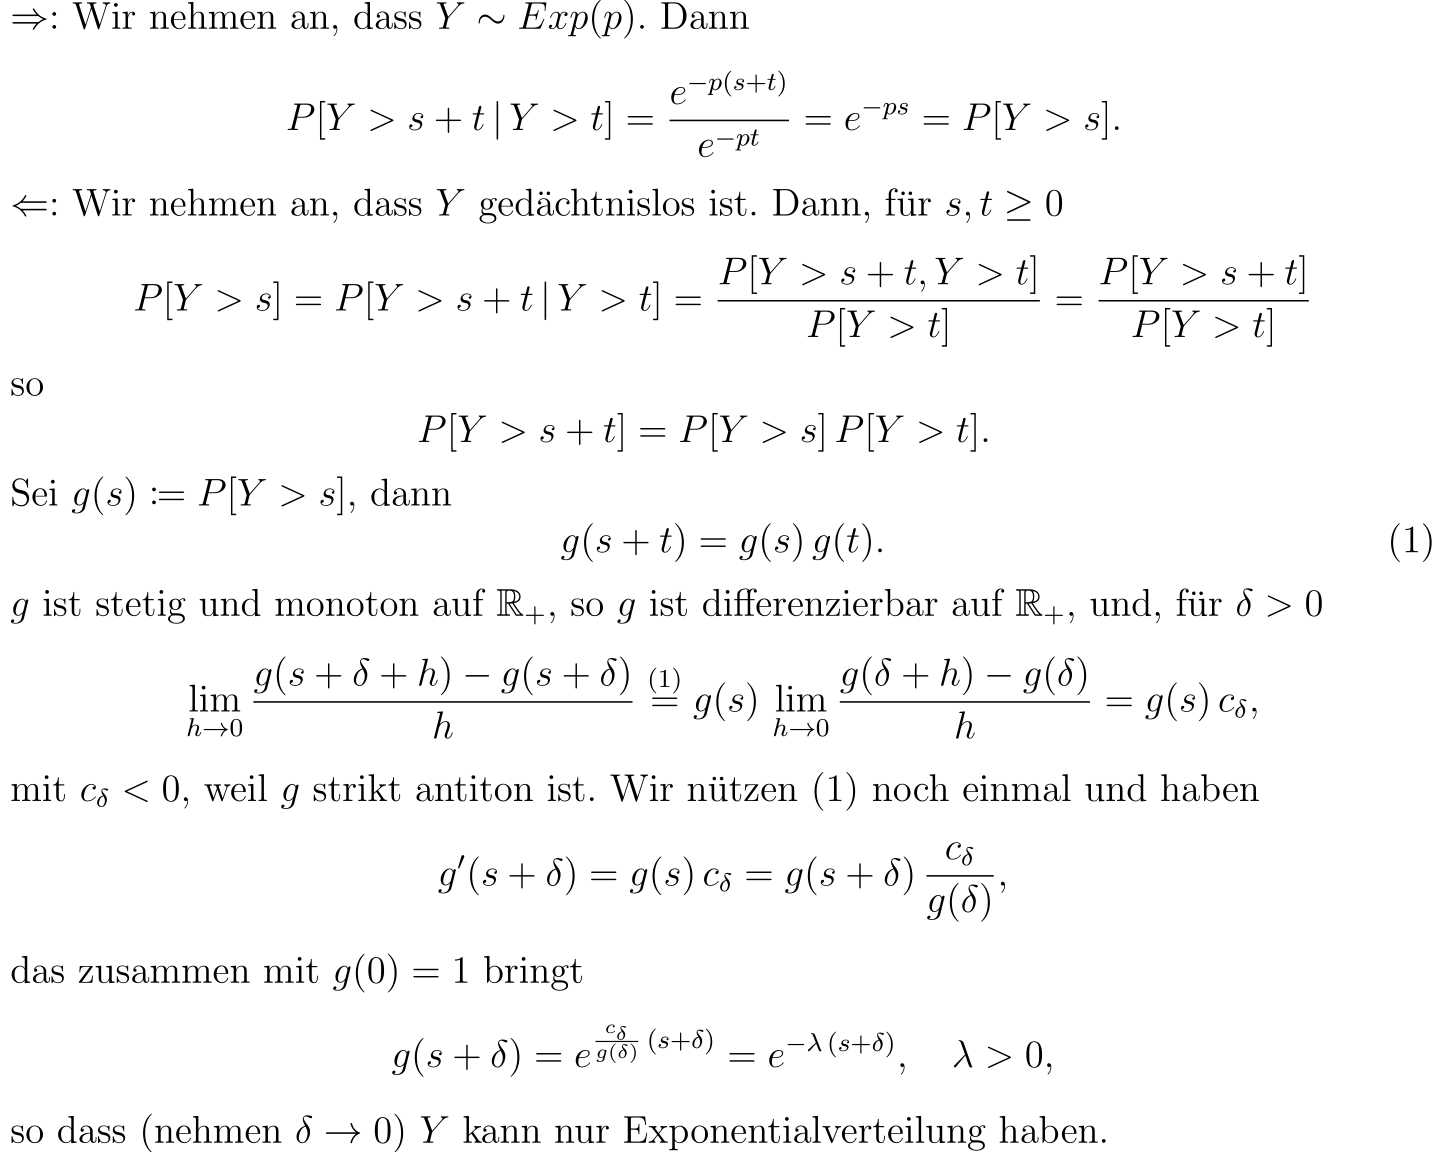
\includegraphics[width=\linewidth]{./Figures/proof_Gedaechnislos.png}

\subsection{Test Nicht Normalverteilt}
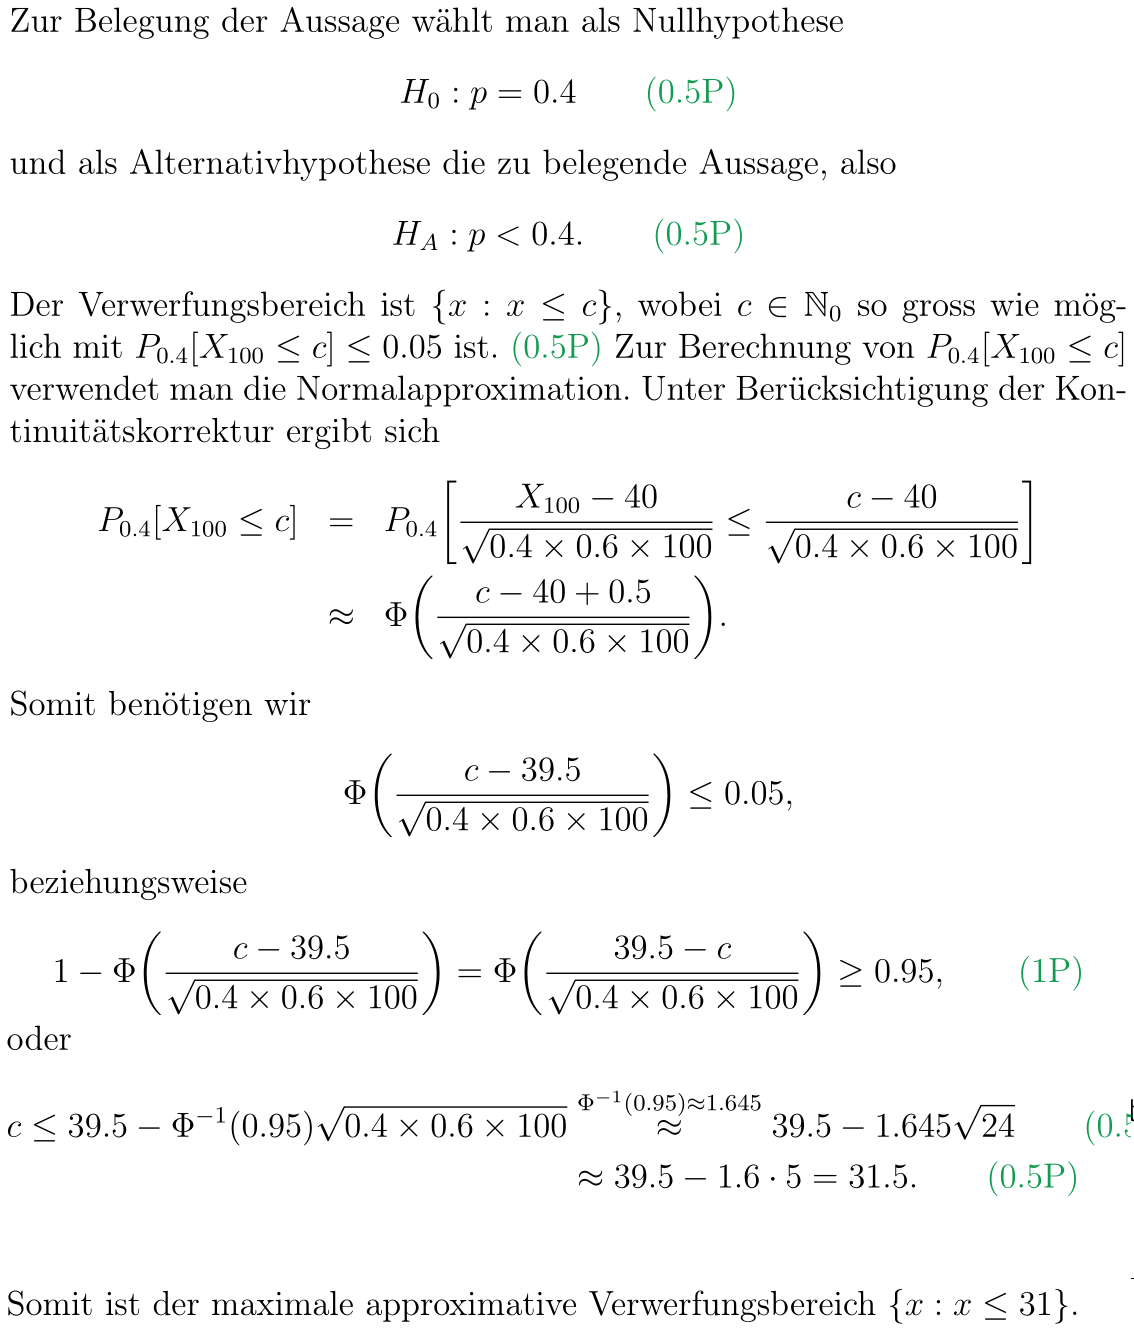
\includegraphics[width=\linewidth]{./Figures/Test_Nicht_Normalverteilt.png}

\subsection{Momenteschätzer}
Für ein Experiment mit $n=5$ unf $f_T(t) = C^2 e^{-Ct} 1_{[0 \le t]}$, bestimme den Momenteschätzer:
\\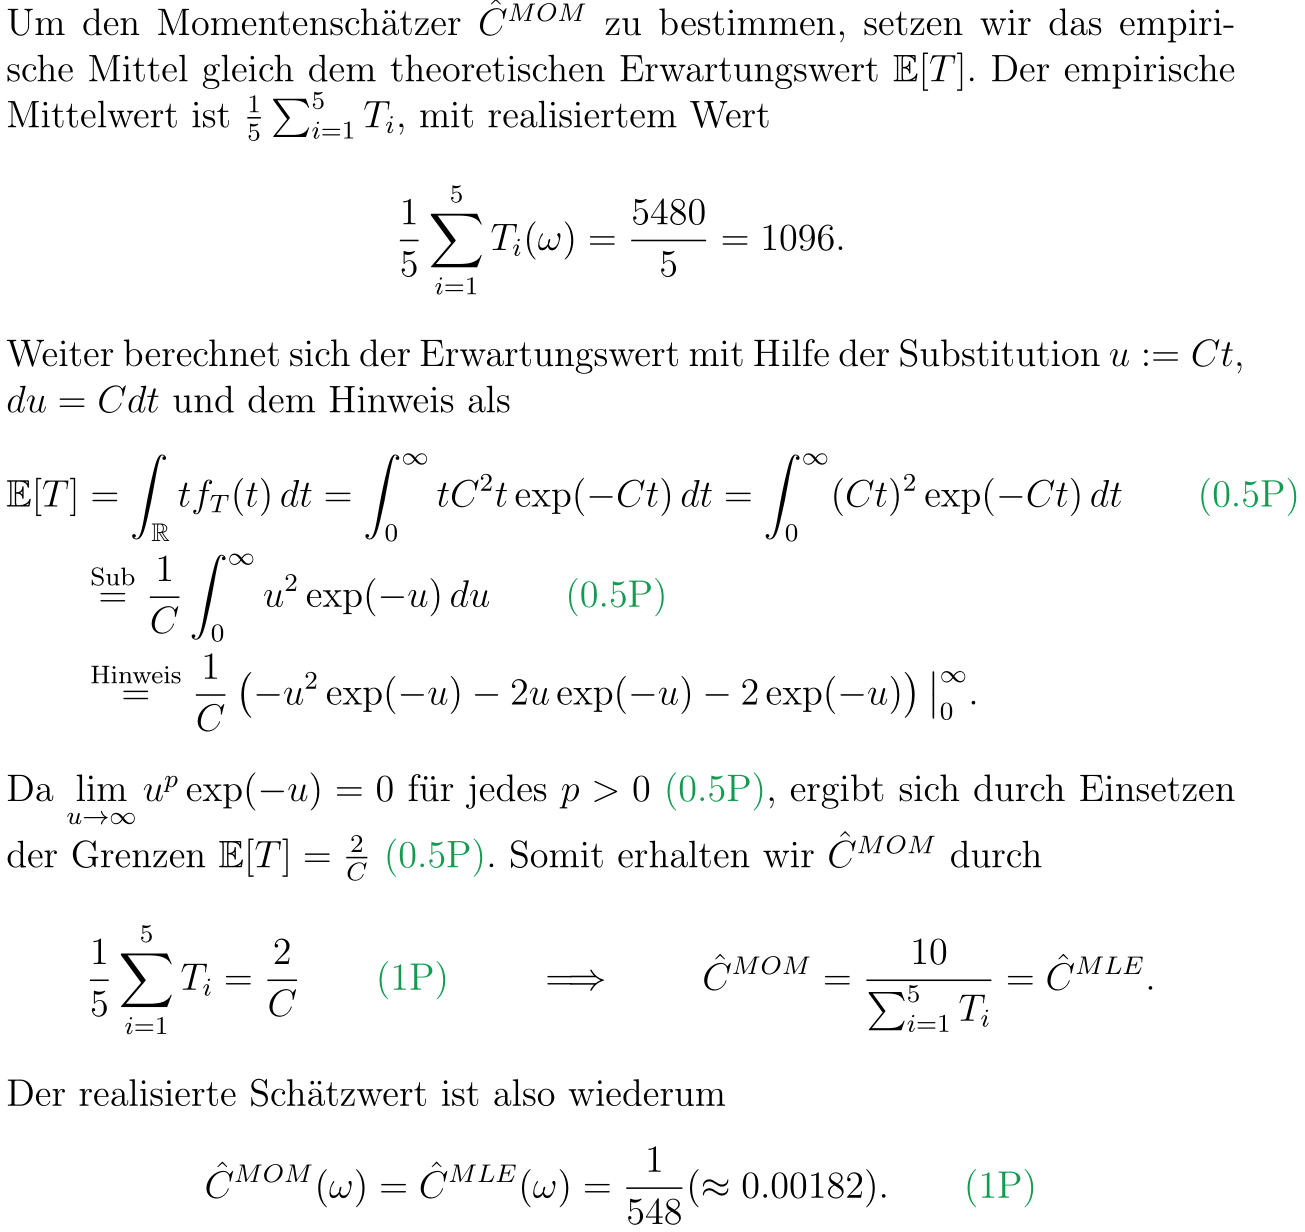
\includegraphics[width=\linewidth]{./Figures/Momente_Schaetzer.png}

\subsection{MinStuff}
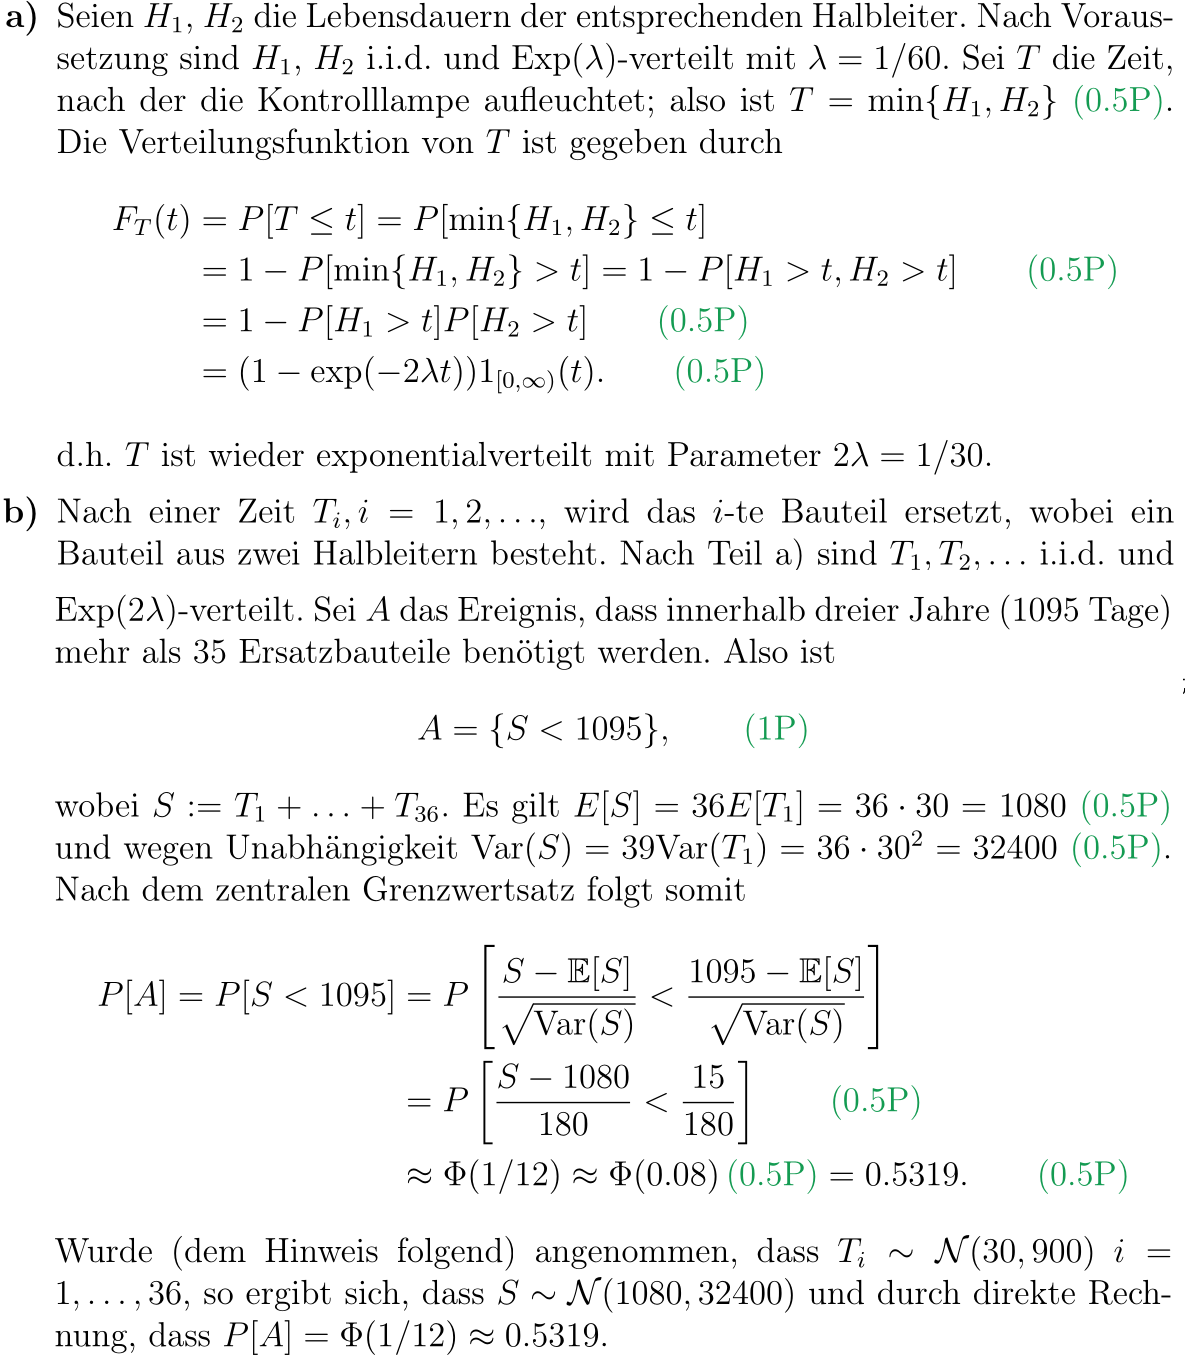
\includegraphics[width=\linewidth]{./Figures/ExampleMinStuff.png}

\subsection{$\chi$ Verteilung}
Für $Y = \sum_{k=1}^v Z_k^2, \quad Z_i \sim \mc{N}(0,1)$ i.i.d. find $E[Y], Var[Y]$:
\\ 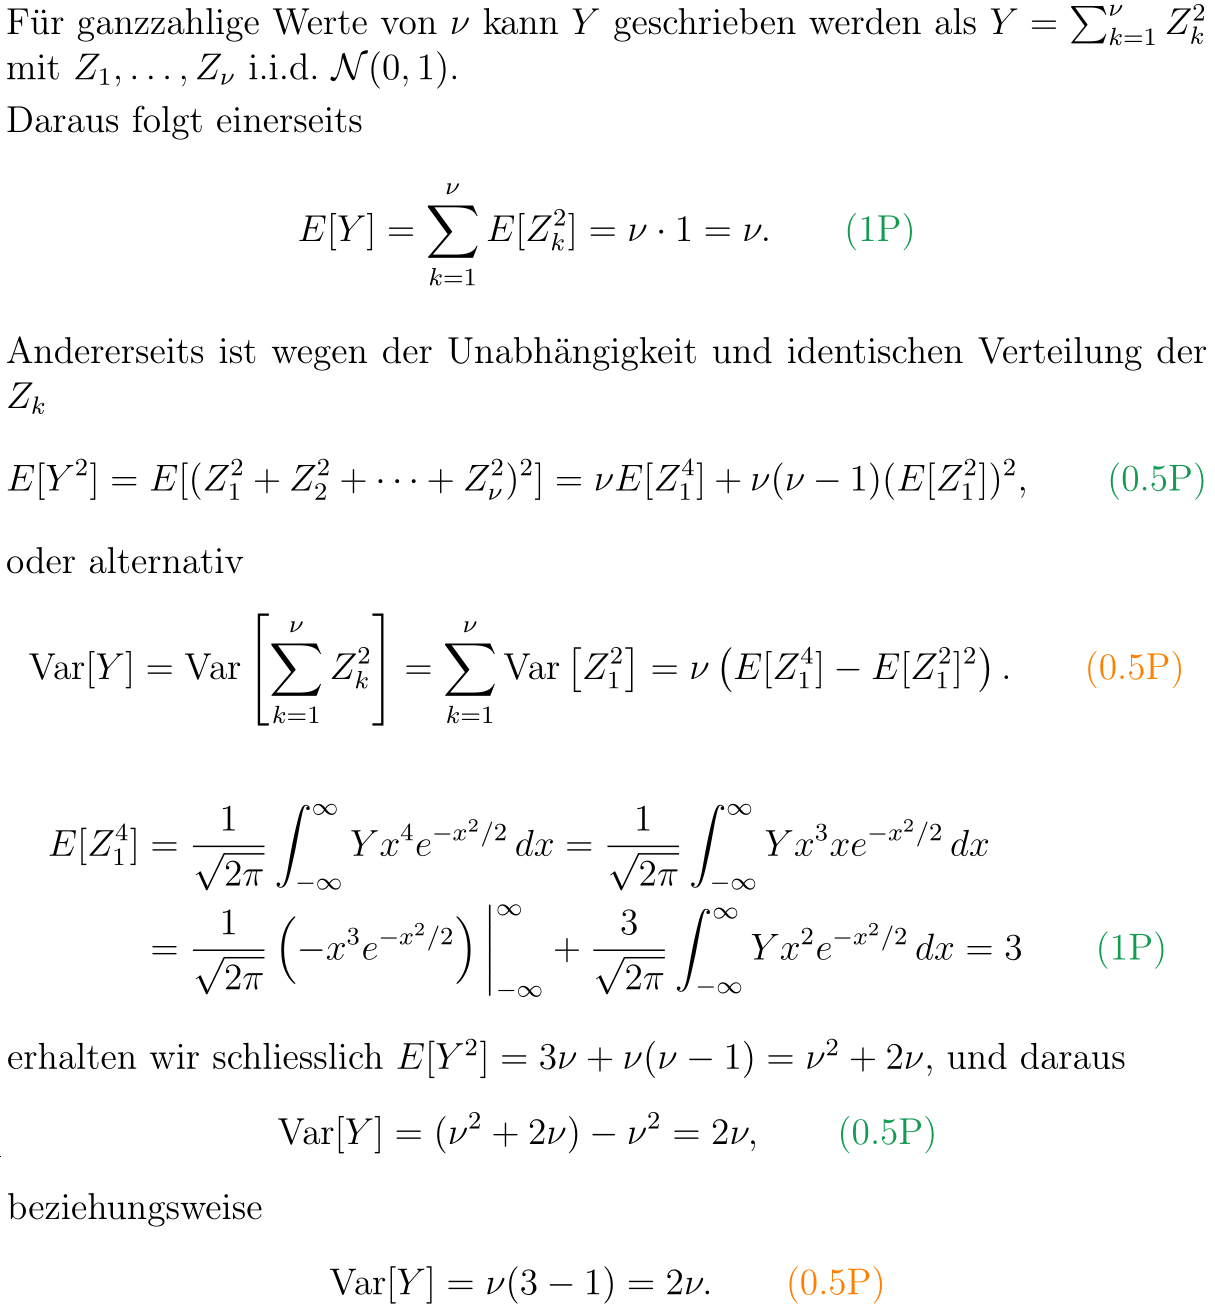
\includegraphics[width=\linewidth]{./Figures/chi_verteilung.png}

\subsection{Grenzwert Überschreitung}
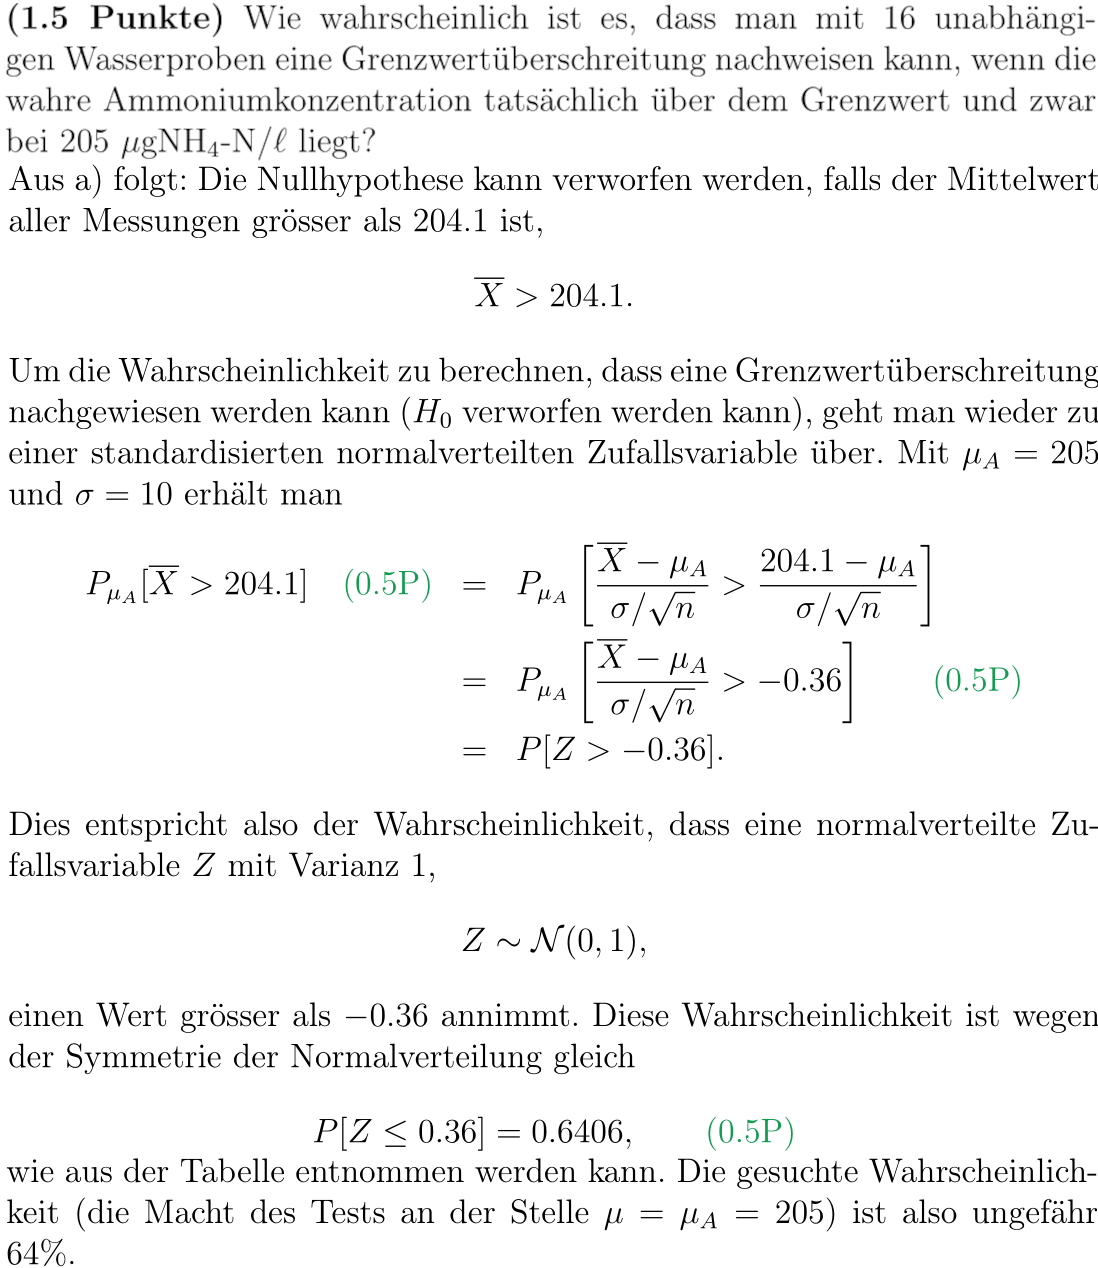
\includegraphics[width=\linewidth]{./Figures/Test_Ueberschreitung.png}

\subsection{Hypergeometrische Verteilung}
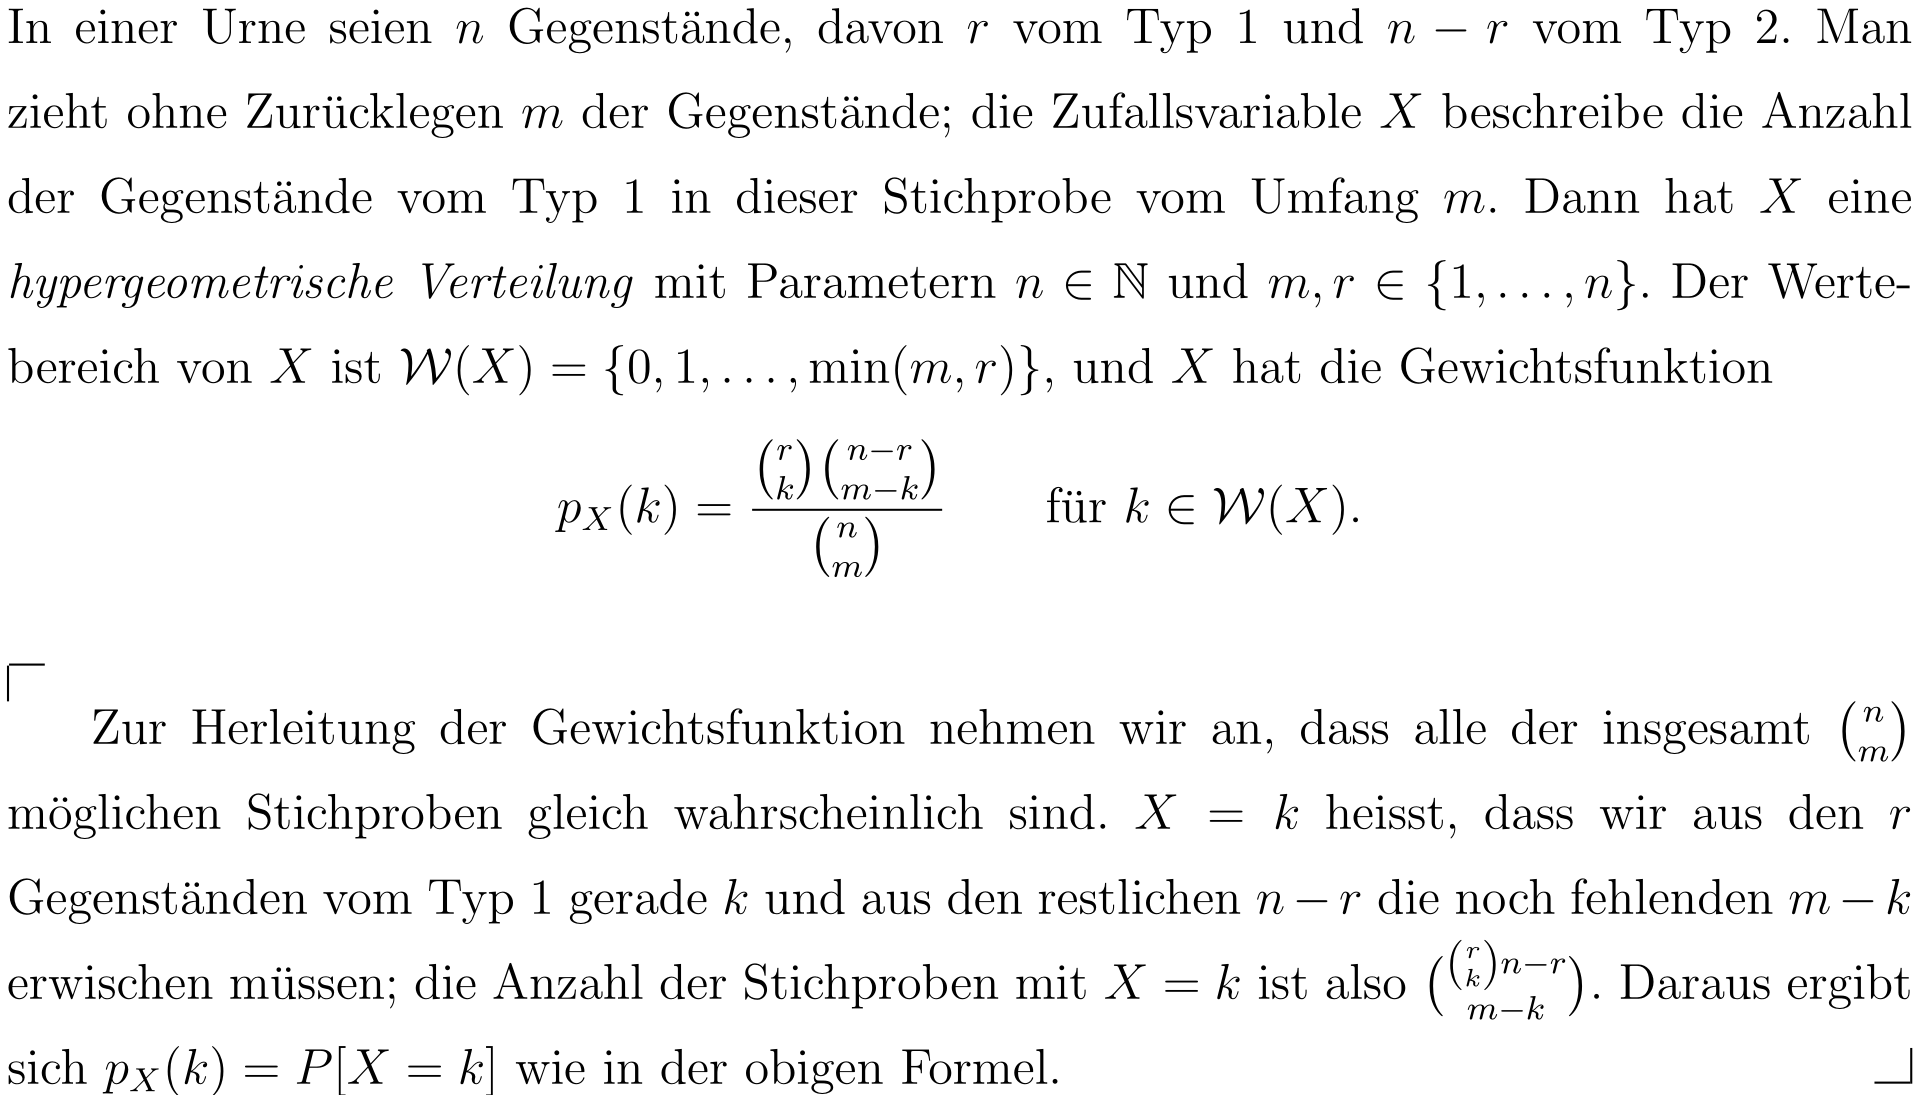
\includegraphics[width=\linewidth]{./Figures/Hypergeometrische_Verteilung.png}

\subsection{Gemeinsame Dichte und Randdichte}
$P \sim \text{Uniform}(0,1), H|P \sim \text{Uniform}(0,P)$, finde:
\begin{itemize*}
    \item Gemeinsame Dichte
    \\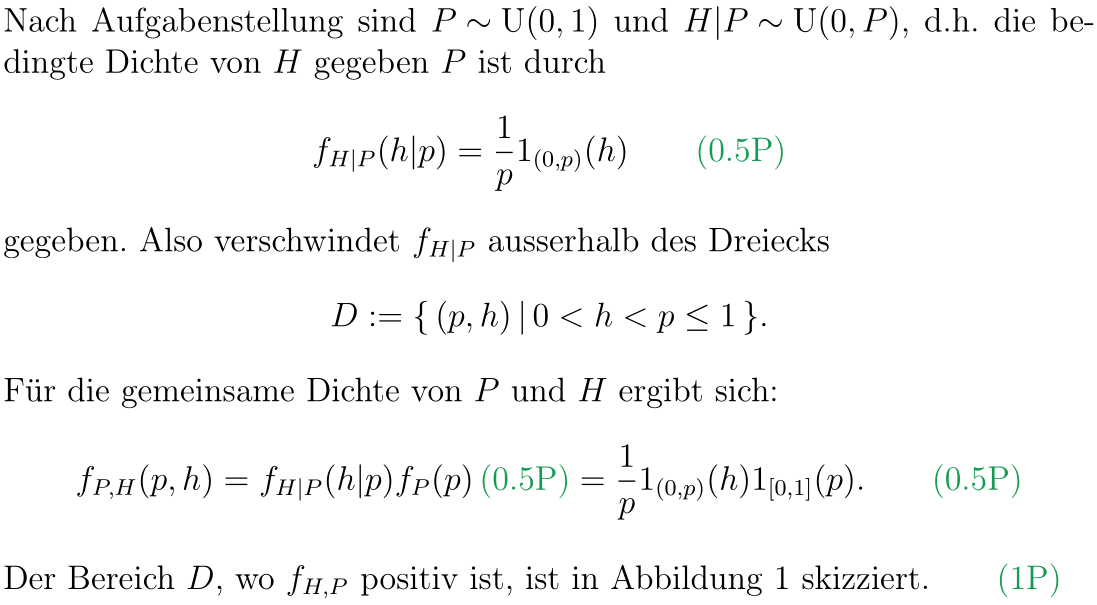
\includegraphics[width=\linewidth]{./Figures/Gemeinsame_Dichte_Randdichte_A.png}
    \item Randdichte von $H$
    \\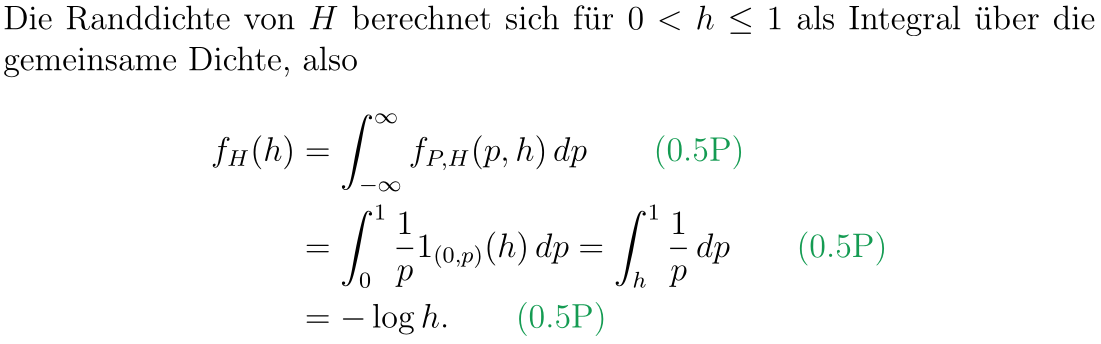
\includegraphics[width=\linewidth]{./Figures/Gemeinsame_Dichte_Randdichte_B.png}
    \item $E[H]$
    \\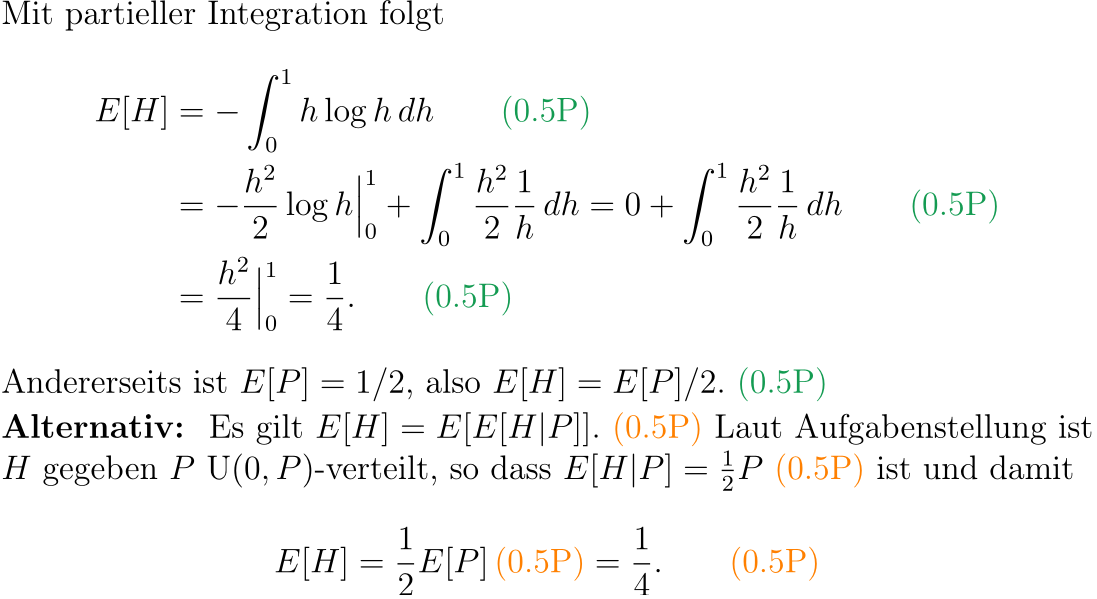
\includegraphics[width=\linewidth]{./Figures/Gemeinsame_Dichte_Randdichte_C.png}
\end{itemize*}

\end{multicols*}
\end{document}
